\documentclass[a4paper,11pt]{report}
\usepackage{geometry}
\geometry{verbose,a4paper,tmargin=25mm,bmargin=25mm,lmargin=25mm,rmargin=25mm}
\usepackage[utf8]{inputenc}
\usepackage[singlespacing]{setspace}
\usepackage{textcomp}
\usepackage{blindtext}
\usepackage{titlesec}
\setlength{\marginparwidth}{2cm}
\usepackage{todonotes}
\usepackage[ngerman]{babel}
\usepackage{listings}
\usepackage{parskip}
\usepackage{verbatim}
\usepackage{graphicx}
\usepackage{chngcntr}
\usepackage{csquotes}
\usepackage[backend=bibtex,citestyle=verbose-ibid]{biblatex}
\usepackage{footnote}
\usepackage[section]{placeins}
\usepackage{algpseudocode}
\usepackage{algorithm}
\usepackage{array}
\usepackage{threeparttable}
\usepackage{pgfplots}
\usepackage{longtable}
\usepackage[automake,acronym,xindy,toc]{glossaries}
\usepackage{hyperref}
\usepackage[ngerman]{cleveref}
\usepackage{makeidx}   % load package



\newcommand*{\bildquelle}[1]{\par\raggedleft\footnotesize Quelle:~#1}


%\newglossaryentry{Canvas}
%{
%name=Canvas,
%description={oder Leinwand. Bezeichnet eine Fläche eines Fensters in der Computergrafik, %%in die virtuell gezeichnet werden kann}
%}


\newacronym{hzb}{HZB}{Helmholtz-Zentrum Berlin}


\makeglossaries
\usepackage[xindy]{imakeidx}
\makeindex




%\addbibresource{bibtex.bib}

\counterwithout{figure}{chapter}
\counterwithout{footnote}{chapter}

\titleformat{\chapter}[display]
   {\normalfont\large\bfseries}
   {\chaptertitlename\ \thechapter}{1em}{\large}
\titleformat{\section}
   {\normalfont\large\bfseries}
   {\thesection}{1em}{}
   
\titleformat{\subsection}
   {\normalfont\small\bfseries}
   {\thesubsection}{1em}{}


\title{Abschlussarbeit Master Medieninformatik}
\author{Viola Jertschat}

\bibliography{references/references}{}

\begin{document}


\begin{titlepage}
	\centering
	
\includegraphics[width=\textwidth]{images/beuthlogo.eps}\par\vspace{1cm}
	{\scshape\LARGE Beuth Hochschule für Technik \par}
	\vspace{1cm}
	{\scshape\Large Abschlussarbeit Master Medieninformatik\par}
	\vspace{1.5cm}
	{\huge\bfseries mARt: Interaktive Darstellung von MRT Daten in AR\par}
	\vspace{2cm}
	{\Large\itshape Viola Jertschat\par}
	\vfill
	betreut von\par
	Prof. Dr.-Ing. Kristian \textsc{Hildebrand}

	\vfill

% Bottom of the page
	{\large \today\par}
\end{titlepage}

\tableofcontents


\listoffigures

\printglossaries

\include{chapters/chapter}
% Related works

\chapter{Verwandte Arbeiten}

\section{Ein Abschnitt}
% Anforderungsanalyse

\chapter{Anforderungsanalyse}
\label{anforderung}

\section{Interviews}

Wie bereits beschrieben, ist es das Ziel dieser Arbeit Neurologen eine dreidimensionale Darstellung von Gehirn-MRT-Scans in einer interaktiven AR- bzw. VR-Anwendung zur Verfügung zu stellen, um zu untersuchen, inwiefern diese die Ärzte in ihrer Arbeit besser unterstützt, als bisher verwendete Darstellungssoftware. Die hypothetischen Vorteile eines solchen Programmes wurden im Kapitel \ref{motivation} erläutert.
Für den Vergleich mit bisheriger Software ist eine Anwendung prototypischen Charakters ausreichend. Diese soll auf die grundlegenden Interaktionen beschränkt sein, die ein Neurologe für die Verarbeitung der Daten benötigt.

Der Fokus der Untersuchung liegt auf dem Bereich der akuten Schlaganfallbehandlung. Wie im Kapitel \ref{grundlagen} beschrieben untersucht der Neurologe hierfür die Abbildungen des Gehirns eines Patienten, die durch den MRT-Scan erzeugt wurden. Dabei hält er nach Bereichen Ausschau, die von einem Schlaganfall betroffen sein könnten, um die Art des Schlaganfalls zu bestimmen, ? sowie den entstandenen Schaden einschätzen zu können. Betroffene Bereiche werden anschließend vom Arzt markiert. Diese Markierung kann danach ein- und ausgeblendet werden.

Um zu bestimmen, welche Interaktionen und Funktionen ein Neurologe benötigt, um effektiv mit der Anwendung arbeiten zu können, wurden iterativ mehrere Interviews mit dem betreuenden Neurologen der Charité Berlin geführt. Die Antworten des Arztes wurden in Anforderungen übertragen, die im folgenden Abschnitt festgehalten wurden. 

\section{Anforderungen als User Stories}

Die im Gespräch mit dem Arzt entwickelten Anforderungen an mARt wurden in Tabelle \ref{tab:userStories} als User Stories.
User Stories werden in der Software-Entwicklung verwendet, um einzelne Funktionen zu definieren, die möglichst unabhängig voneinander implementiert werden können sowie mehr aus Sicht des Nutzers zu denken, statt aus der Sicht des Entwicklers (\cite{UserStoriesApplied)}.
Zur besseren Referenzierung wurden die Stories jeweils mit Bezeichnern versehen. Da viel der Interaktionen sowohl für die zwei- als auch dreidimensionale Darstellung benötigt werden wurde weiterhin gekennzeichnet, welche Darstellung von der jeweiligen Story betroffen ist.

\begin{longtable} {p{.125\textwidth}p{.50\textwidth}p{.05\textwidth}p{.225\textwidth}}
\toprule
Bezeichnung & User Story & 2D/3D & Anforderungsreferenz \\
\toprule
U01 & Als Nutzer möchte ich eine möglichst genaue und gut erkennbare Abbildung der MRT-Bilder, damit ich eine Vorstellung habe, wie das Gehirn des Patienten aussieht. & beide & A05\\
\midrule 
U02 & Als Nutzer möchte ich die Daten als zweidimensionale Schichten aus mindestens einem Winkel betrachten können, um diese wie gewohnt untersuchen zu können.  & 2D & A02\\
\midrule 
U03 & Als Nutzer möchte ich die Daten als dreidimensionales Volumen betrachten können, um ein besseres Verständnis für den Zustand des Gehirns zu erhalten. & 3D & A02\\
\midrule 
U04 & Als Nutzer möchte ich mindestens zwei Datensätze nebeneinander anzeigen lassen, um direkte Vergleiche zwischen diesen ziehen zu können. & beide & A14\\
\midrule 
U05 & Als Nutzer möchte ich aus verschiedenen Datensätzen auswählen können, welche angezeigt werden, um mich auf die relevanten Daten konzentrieren zu können. & beide & A01\\
\midrule
U06 & Als Nutzer möchte ich entscheiden können, ob ich mehrere angezeigte Datensätze gleichzeitig oder einzeln manipuliere (z.B. Kontrast), um die Einstellungen genau an jeden Datensatz anpassen zu können. & beide & A14\\
\midrule 
U07 & Als Nutzer möchte ich auf mindestens einer Achse durch beide Darstellungen scrollen können, um das Innere des Organs zu untersuchen. & beide & A04\\
\midrule 
U08 & Als Nutzer möchte ich mit einem Scrollrad durch die Darstellungen scrollen können, um genaue Kontrolle darüber zu haben, welche Schichten angezeigt werden. & beide & A11\\
\midrule 
U09 & Als Nutzer möchte ich zwischen einer zwei- und dreidimensionalen Darstellung der Daten wechseln können, um die Vorteile beider Darstellungen für meine Untersuchung zu nutzen. & beide & A02\\
\midrule 
U10 & Als Nutzer möchte ich, dass bisherige Manipulationen beim Wechsel zwischen 2D und 3D übernommen werden, um die Orientierung und Sichtbarkeit zu erhalten. & beide & A13\\
\midrule 
U11  & Als Nutzer möchte ich den gekennzeichneten vom Schlaganfall betroffenen Bereich ein- und ausblenden können, um mich auf diesen, oder die Darstellung an sich konzentrieren zu können. & beide & A02\\
\midrule
U12 & Als Nutzer möchte ich auch dann noch die Strukturen des Gehirns erkennen, wenn der gekennzeichnete Bereich eingeblendet ist. & beide & A03\\
\midrule 
U13 & Als Nutzer möchte ich die MRT-Darstellungen drehen können, um den besten Blickwinkel auf den für mich relevanten Bereich zu bekommen. & 3D & A09\\
\midrule 
U14 & Als Nutzer möchte ich die Helligkeit und den Kontrast der Darstellung verändern können, um Strukturen besser deutlich zu machen. & beide & A09\\
\midrule 
U15 & Als Nutzer möchte ich die MRT-Darstellungen skalieren können, um die Darstellung gut zu erkennen. & beide & A08\\
\midrule 
U16 & Als Nutzer möchte ich die MRT-Darstellungen frei im Raum bewegen können, um sie meiner Position anzupassen. & beide & A07\\
\midrule 
U17 & Als Nutzer möchte ich, dass das Hologram seine Position im Raum behält, um es von allen Seiten betrachten zu können. & beide & A13\\
\midrule 
U18 & Als Nutzer möchte ich alle vorhandenen MRT-Sequenzen sehen und zwischen ihnen wählen können, damit ich alle notwendigen Informationen zu dem Scan nutzen kann. & beide & A12\\
\midrule 
U19 & Als Nutzer möchte ich Dateien im NIfTI-Format in der Anwendung verwenden können, damit ich sie nicht vorher umwandeln muss. & beide & A13\\
\midrule 
U20 & Als Nutzer möchte ich Dateien im DICOM-Format in der Anwendung verwenden können, damit ich sie nicht vorher umwandeln muss. & beide & A13\\

\bottomrule
\caption{\label{tab:userStories}Aus Interviews abgeleitete User Stories.}
\end{longtable}


% Konzept

\chapter{Konzept}
\label{konzept}

Im folgenden werden Konzepte diskutiert, um die in Kapitel \ref{anforderung} herausgearbeiteten Anforderungen zu erfüllen.

\section{Implementierungsziele}
Ziel des Arbeit ist es eine prototypische AR- bzw. VR-Anwendung zur Visualisierung und Untersuchung von MRT-Daten zu implementieren. 

Vor allem im Bereich der Volumendarstellung gibt es bereits viele Programme und Arbeiten, die diese erfolgreich umsetzten, wie im Kapitel \ref{grundlagen} erläutert wurde.
Wie später beschrieben wird, baut mARt auf einer bereits implementierten Lösung auf. Die Anwendung soll mit der Spiele-Engine \textit{Unity}  implementiert werden, worauf ebenfalls im späteren Kapiteln eingegangen wird. Die Implementierung muss also mit der Software kompatibel sein. In Kapitel \ref{grundlagen} wurde unter anderem die \textit{Unity}-Erweiterung \textit{Volume Viewer Pro} beschrieben, die viele der gestellten Anforderungen bereits abdeckt. Das Programm ist allerdings kostenpflichtig. Eine unabhängige und frei zugängliche Software ist dem vorzuziehen. Vor allem, da es sich um einen Prototyp handelt, der Aufschluss über die Verwendungsmöglichkeiten in diesem Bereich liefern und daher eventuell weiterentwickelt werden soll. Deshalb sollte die dreidimensionale Darstellung im Rahmen dieser Arbeit entwickelt werden und Code aus anderen Quellen nur verwendet werden, wenn er diesen Kriterien (z.B. lizenzrechtlichen Bestimmungen) entspricht.

Weiterhin soll die Darstellung in eine interaktive Anwendung eingebettet sein, die die in Kapitel \ref{anforderung} formulierten Anforderungen erfüllt.

\section{3D Darstellung}
\label{3dDarstellung}

Im Kapitel\ref{grundlagen} wurden verschiedene Methoden vorgestellt, um ein Volumen zu visualisieren. An dieser Stelle soll diskutiert werden, welche davon sich am besten für die Umsetzung in mARt eignet.
Die 3D-Darstellung sollte die in Kapitel \ref{anforderung} beschriebenen Eigenschaften haben:

\begin{itemize}
\item Darstellung sollte das Volumen dreidimensional abbilden. \textbf{(U03)}
\item Die innere Struktur des Gehirns sollte erkennbar sein \textbf{(U01)}
\item Die Markierung des vom Schlaganfall betroffenes Bereichs sollte die MRT-Darstellung nicht unkenntlich machen. \textbf{(U12)}
\item Es sollte möglich sein durch die Schichten des Volumes zu scrollen. \textbf{(U07)}
\end{itemize}

Dadurch lassen sich Aussagen über das gewünschte Aussehen der Darstellung herleiten.
Da das Innere der 3D Darstellung erkennbar sein soll, muss eine semi-transparente Darstellung erzeugt werden, die sowohl die Form des Gehirns abbildet, als auch die innere Struktur. Die eingeblendete Markierung sollte ebenfalls zu einen gewissen Grad transparent sein.
Weiterhin sind sind nur die Pixel relevant, die das Gehirn darstellen. Der Bereich darum (Schädel und Hintergrund) sollten gefiltert  und nicht sichtbar gemacht werden. Das gewünschte Ergebnis ist, dass das Gehirn frei im Raum schwebt. 

Die Anforderungen sprechen gegen eine Umsetzung, die eine Oberfläche des Gehirns erzeugt und es als Mesh darstellt. Die Form des Gehirns könnte dadurch deutlich gezeigt werden und das Objekt würde von den umgebenden Pixeln getrennt werden. 
Allerdings handelt es sich bei dem Gehirn nicht um eine Hülle sondern eine Masse. Es ist unwahrscheinlich, dass ein Verfahren wie Marching Cubes die inneren Gehirnstrukturen exakt genug wiedergeben könnte, damit ein Neurologe sinnvolle Schlüsse daraus ziehen kann. Die binäre Aufteilung der Voxel kann außerdem dazu führen, dass Teile des Gehirn fehlerhafter Weise nicht angezeigt werden. Weiterhin müsste das Mesh in Echtzeit kontinuierlich angepasst werden, wenn der Nutzer durch die verschiedenen Schichten scrollt. 
Deshalb eignet sich eine Oberflächengenerierung nicht zur Visualisierung.
Hinzu kommt, dass in den Anforderungen kein Anwendungsfall beschrieben wird, der eine Oberfläche erfordert, wie z.B. die Berechnung einer Kollision des Gehirns mit einem anderen Objekt.	
	
Die dreidimensionale Darstellung lässt sich demnach besser mit einer Volume Rendering Methode umsetzten.  
In Kapitel \ref{grundlagen} wurden die verschiedenen Volume Rendering Techniken miteinander verglichen.
Die Visualisierung der MRT-Daten wurde im Rahmen dieser Arbeit mit den Volume Raycasting Verfahren umgesetzt.
Das Raycasting Verfahren liefert die beste Bildqualität, wie aus dem Vergleich hervorgeht. Es ist daher auch weit verbreitet bei der Implementierung von Volume Rendering Software, wie in Abschnitt \ref{volumeRenderingImplementierung} gezeigt wurde. 
Die verschiedenen Implementierungen können zur Orientierung und als Referenz für die eigene Umsetzung verwendet werden.
Die Technik lässt sich außerdem gut durch einen Fragment-Shader realisieren was eine Implementierung in \textit{Unity} erleichtert. 
Das für Texture-Based Rendering benötigte Texture Slicing und Mapping ist in der Umsetzung nicht trivial und die Ergebnisse des Verfahrens rechtfertigen diesen Aufwand nicht.
Obwohl die Shear-Warp Methode in der Theorie ähnlich abläuft wie das Raycasting, ist die Implementierung komplexer.
Für eine Umsetzung des Volume Renderings im Rahmen dieser Arbeit eignet sich das Raycasting Verfahren deshalb am besten.
Zwar ist die Berechnung einzelner Strahlen leistungsintensiv, kann aber durch Optimierungen und die Verwendung von passender Hardware trotzdem in Echtzeit und interaktiv realisiert werden.

Weiterhin wurden in Abschnitt \ref{klassifikation} die verschiedene Arten erläutert eine Klassifikation zu implementieren. Durch die Umsetzung im Fragment-Shader wird eine Post-Klassifikation umgesetzt. 
Von der Umsetzung einer Pre-Integrierten Klassifikation wurde abgesehen. Zum Einen auf Grund des zusätzliche Implementierungsaufwands, zum Anderen weil die Renderings keine schwerwiegenden Artefakte aufwiesen. Letzteres wird im Abschnitt \ref{ergebnisse} aufgegriffen.

Wie im Kapitel \ref{grundlagen} beschrieben, werden beim Volume Rendering in der Regel Transferfunktionen eingesetzt, um verschiedene Gewebestrukturen oder Materialien zu unterscheiden. Dabei handelt es sich um eine Look-Up-Tabelle in Form einer Textur, die jedem Isowert eine Farbe und Opazität zuweist.
Die Herausforderung bei der Implementierung einer Transferfunktion ist dabei die Generierung einer zum Datensatz passenden Textur. Selbst bei einer Transferfunktion mit nur einer Dimension müssen häufig verschiedene Wertzuweisungen ausprobiert werden, um ein gutes Ergebnis zu erhalten.
Um eine bzw. mehrere Transferfunktionen zu generieren, die den Ansprüchen des Nutzers genügt und die für verschiedene Datensätze passend sind, ist es deshalb sinnvoll dem Nutzer eine Benutzeroberfläche zur Verfügung zu stellen, mit deren Hilfe er die verwendete Transferfunktion zur Laufzeit manipulieren kann. 

In einem Volumen gibt es in der Regel bestimmte Isowerte, die Grenzwerte zwischen verschiedenen Materialien darstellen. Diese dienen als Kontrollpunkte zwischen denen interpoliert wird, um einen Farbverlauf zwischen den Materialien zu erhalten. 
Um die Transfertextur zu beeinflussen muss der Nutzer diese Kontrollpunkte verändern können. Er muss dabei für jeden Kontrollpunkt dessen Iso-, Farb- und Opazitätswert festlegen. Zwischen den Werten der Kontrollpunkte kann dann eine Spline-Interpolation stattfinden.
Die nutzergesteuerte Generierung von Transferfunktionen konnte aus zeitlichen Gründen im Rahmen dieser Arbeit nicht umgesetzt werden.


\section{Darstellung des gekennzeichneten Bereichs}
\label{maske}


In User Story \textbf{U11} der Anforderungen wird beschrieben, dass der vom Schlaganfall betroffene Bereich des Gehirns, der vorher von einem Arzt gekennzeichnet wurde in der Darstellung angezeigt werden soll, wenn dies gewünscht wird. 
Der Bereich wird durch Masken definiert, die zuvor von einem Arzt in einem externen Programm erstellt wurden und ebenfalls im NIfTI-Format vorliegen. Für jede Schicht in einem Datensatz existiert ebenfalls eine Schicht im Maskendatensatz. 

Der Bereich soll sowohl in der zwei- als auch in der dreidimensionalen Ansicht dargestellt werden. Bei letzterer sollte er auch in den Querschnitten erkennbar sein, die sich durch das Scrollen durch das Volumen ergeben. MRT-Daten und markierter Bereich verhalten sich also gleich.

Da die Daten im selben Format vorliegen und sich gleich verhalten sollen, ist es naheliegend, dass sie auf die selbe Weise gerendert werden. Dementsprechend werden auch die Maskenbilder in eine 3D-Textur übertragen, die dann durch Volume Raytracing gerendert wird. Damit aber nicht jeder Strahl doppelt verschossen werden muss, der das Volumen durchdringt, wird der Zugriff auf die Maskentextur in den Shader integriert, der bereits das MRT-Volumen rendert. Für jeden Voxel, der aus der 3D-Textur der MRT-Daten gelesen wird, wird  der Voxel mit denselben Koordinaten aus der Masken-3D-Textur gelesen. Die zwei Farbwerte werden zum Schluss miteinander verrechnet. Durch die Verrechnung, bleibt trotzdem die Struktur des Gehirns erkennbar, wie es von \textbf{U12} gefordert wird. Die Abfrage der Maskenwerte erfolgt nur, wenn durch das Material eine entsprechende Steuervariable gesetzt wurde.
Dies wird im folgenden Codebeispiel veranschaulicht.

\begin{listing}[!htb]
\begin{minted}[mathescape,
               linenos,
               numbersep=5pt,
               gobble=2,
               frame=lines,
               framesep=2mm]{csharp}
void main(sampler3D _Volume,
		  sampler3D _MaskVolume,
          sampler1D _TransferTexture,
          float3 texCoord : TEXCOORD0,
          float4 maskColor : COLOR,
          float _ShowMask)
          {
          
          	// Isowert des Volumens wird für die aktuelle Position ausgelesen
          	float isoValue = tex3D(_Volume, texCoord);
          
          	if (_ShowMask == 1)
          	{
          		// Isowert des Maskenvolumens wird für die 
          		// aktuelle Position ausgelesen
          		float isoValueMask = tex3D(_MaskVolume, texCoord);
          	
          		// Die Maske wird eingefärbt
          		isoValueMask *= maskColor;
          	}
          
          	// Die Werte werden verrechnet
          	return isoValue * isoValueMask;
          }
\end{minted}
\caption{Bestimmung der Farbe eines Pixels in Abhängigkeit zum entsprechenden Isowert sowie dem Iso- und Farbwert der Maskentextur. Letztere werden nur angewandt, wenn die Steuervariable dafür gesetzt wurde. Selbst erstelltes Beispiel}
\label{lst:transfer}
\end{listing}
\FloatBarrier

\section{2D Darstellung}

Neben der dreidimensionalen Ansicht sollen die Daten auch in zwei Dimensionen untersucht werden können, wie es auch in vielen Bildschirmanwendungen der Fall ist.
Die Betrachtung von jeweils nur einer Schicht des Datensatzes erlaubt es den Fokus auf bestimmte Merkmale oder Regionen zu legen, die in dieser Darstellung deutlicher sein könnten als in der volumetrischen. Weiterhin wird der direkte Vergleich zwischen den Szenen deutlicher. Beispielsweise kann die Annahme von der Größe eines Bereichs in der 3D-Darstellung überprüft und so eventuell korrigiert werden.

Da in User Story \textbf{U02} nur das Scrollen auf einer Achse durch die Bildschichten gefordert wird, wird jeder Datensatz als quadratische Bildfläche dargestellt.
Die Anzeige der Daten aus verschiedenen Sichtachsen wäre nicht nur aufwändiger in der Umsetzung, sondern würde die Komplexität der Anwendung auch deutlich steigern, wodurch ihre Benutzbarkeit sinken könnte. 

Die zweidimensionale Darstellung in mARt kann kaum einen Mehrwert gegenüber einer Bildschirmanwendung  bieten. Zwar kann sie zur Untersuchung der Daten genutzt werden, dient allerdings hauptsächlich als komplementäre Ansicht zur 3D-Visualisierung.

\section{Endgerät}
\label{device}

Wie bereits im Abschnitt \ref{motivation} beschrieben, ist mARt als AR-HMD-Anwendung konzipiert. Obwohl die Technologie noch viele Unzulänglichkeiten aufweist, eignet sie sich auf lange Sicht dennoch besser für den Einsatz in einem medizinischen Arbeitsumfeld.
Für den Arbeitsalltag eines Arztes und die Zusammenarbeit mit Patienten eignet sich ein durchsichtiges Display deutlich besser als ein undurchsichtiges. Der Nutzer verliert somit nicht seine Umwelt aus den Augen, wodurch er sich sicherer in der Benutzung fühlt. In einem Anwendungsszenario, in dem er mit anderen Menschen kommuniziert, während er die Anwendung bedient, gilt dies umso mehr. Die mögliche Verwendung von mARt während einer Operation oder Behandlung wäre mit einer VR-Anwendung oder Smartphone-App unmöglich. Die Reduzierung auf die virtuelle Realität bietet zudem keinen Vorteil für die Funktion der Anwendung, da die Umwelt in der Anwendung nicht verändert werden soll. 

Ein weiterer Vorteil eines AR-HMDs ist seine Portabilität. Dies ist vor allem entscheidend, wenn die Daten anderen Personen, wie z.B. Patienten gezeigt werden sollen. Das Gerät lässt sich einfach in ein anderes Zimmer mitnehmen, was mit einem VR-System deutlich schwieriger umzusetzen ist.
 
Eine große Einschränkung bietet die geringe Anzahl an Gesten und Interaktionsmöglichkeiten, die die bisherige AR-Technik zur Verfügung stellt. Dies ist allerdings hinfällig, wenn stattdessen die \textit{Leap Motion} verwendet wird, um Nutzereingaben zu erfassen. Die Vorteile des Gerätes werden im folgenden Abschnitt erläutert.

Es ist zu erwarten, dass sich AR-HMDs in den folgenden Jahren deutlich verbessern werden, was Tragekomfort und Leistungfähigkeit angeht. Da mARt als Prototyp einer medizinischen Anwendung anzusehen ist, kann davon ausgegangen werden, dass bei einer Weiterentwicklung der Anwendung Technologie zur Verfügung steht, die viele der genannten Mängel behebt.

Eine AR-Anwendung eignet sich demnach besser für die Umsetzung. Um diese wiederzugeben wurde die \textit{HoloLens} von \cite{hololens} gewählt, da sie bereits 2015 erschienen und verfügbarer ist.
Die Leistung des Gerätes ist allerdings nicht ausreichend, um die intensiven Berechnungen durchzuführen, die für das Volume Raycasting erforderlich sind. Auch der Einsatz der \textit{Leap Motion} erfordert eine hohe Rechenleistung.
In einer Demo, in der das Volume Rendering auf der \textit{HoloLens} getestet wurde, wurde eine Framerate von 2-10 FPS gemessen, wobei die höhere Rate nur bei einer Darstellung mit kleiner Skalierung erreicht wird. \cite{fpsHololens} empfiehlt eine Framerate von 60 FPS, um die beste Erfahrung zu bieten.
Die Framerate ist nicht ausreichend, um eine angenehme und effektive Arbeitsweise zu ermöglichen. 
Hinzu kommt, dass der Einsatz der \textit{Leap Motion} es verhindert, dass die Anwendung für die \textit{HoloLens} bereitgestellt wird. Dies wird in Abschnitt \ref{kombination} erläutert. Die Anwendung wird deshalb lediglich an die \textit{HoloLens} übertragen, was allerdings eine Latenz mit sich bringt. 
Um im Test eine stabile Darstellung und Interaktion zur Verfügung stellen zu können, wurde die Anwendung zusätzlich als VR-Anwendung umgesetzt. Die Funktionalität bleibt dabei gleich. 
Durch Verwendung der \textit{Leap Motion} ist die Interaktion mit dem Modell in beiden Anwendungen identisch. 
Zur Wiedergabe der VR-Awendung wird die \textit{HTC Vive} verwendet.
% Bezug Hololens2?

\section{Interaktionsdesign} 

In diesem Abschnitt wird das Konzept der Interaktion innerhalb der Anwendung beschrieben. Dazu wird zunächst diskutiert, mit welcher Technik die Nutzereingabe erfasst werden soll. Dann wird auf die Gestaltung der Bedienelemente in der Anwendung eingegangen.

\subsection{Nutzereingabe}
%\todo{Referenzen?}

Wie bereits im vorherigen Abschnitt erwähnt, wird die \textit{Leap Motion} in Kombination mit dem jeweiligen HMD benutzt, um den Nutzer mit der Anwendung interagieren zu lassen. 
Die \textit{Leap Motion} verfolgt die Hände des Nutzers und stellt diese als 3D-Modelle innerhalb der Anwendung dar. Die Bewegungen der Hände werden dabei genau nachempfunden, sodass die Illusion entsteht die simulierten Hände wären die eigenen. 
Bereits \cite{Zimmerman86} haben die Hand als natürlichstes Mittel zur Manipulation von Objekten bezeichnet. Zudem haben \cite{Bianchi-Berthouze07} festgestellt, dass Körperbewegung in einer Anwendung zu einem höheren Einsatz in deren Umgang führt. Indem es die Hand in den virtuellen Raum überträgt, fördert die \textit{Leap Motion} den intuitiven Umgang mit der Anwendung enorm und ermöglicht damit ein positives Nutzungserlebnis. Weiterhin wird dadurch das erlernen komplexer Gesten oder die Verwendung von Controllern umgangen. Beides sind Hindernisse, die Nutzer, die mit der Technik nicht vertraut sind abschrecken könnten. 
Nachteilig ist, dass das Sichtfeld der Kamera begrenzt ist. Da diese vorne auf dem HMD angebracht ist, wird dieses noch weiter nach vorne verschoben. Damit seine Hände erkannt werden, muss der Nutzer sie deshalb in einiger Entfernung genau vor sein Gesicht halten. 
Dafür bietet die \textit{Leap Motion} mehr Freiheit in der Interaktion. Dies gilt besonders im Vergleich zu den Eingabemöglichkeiten der \textit{HoloLens}, 
deren Gestenerkennung stark begrenzt ist. Um alle notwendigen Manipulationen der Darstellungen abzudecken, müssten daher entweder deutlich mehr Bedienelemente eingebaut werden oder die Interaktion müsste zu großen Teilen auf Sprachsteuerung beruhen. 
Dies wurde durch Implementierung einer prototypischen \textit{HoloLens}-Anwendung bestätigt, die nur durch die \textit{HoloLens}-Gesten gesteuert werden kann. Sie ist im Kapitel \ref{implementierung} genauer beschrieben.
Ein auf Sprachsteuerung beruhendes Programm ist im Arbeitsalltag eher umständlich, vor allem wenn sich der Anwender im selben Raum wie andere Personen befindet. Zudem wirft es die Problematik der Mehrsprachigkeit auf. 
Allerdings wurde im Frühjahr 2019 ein Nachfolgemodell der \textit{HoloLens} angekündigt, das alle Handbewegungen des Nutzers verfolgt und somit auch Gesten wie Greifen erkennt. Dies wird noch einmal in Abschnitt \ref{hololens2Fazit} erläutert. Es zeigt, dass eine Steuerung durch die Hände des Nutzers nicht nur sinnvoll ist, sondern in der Zukunft auch durch ein HMD umgesetzt werden kann.

Da mARt schließlich in Form einer AR- und VR-Anwendung umgesetzt wird stellt sich weiterhin die Frage nach den Bedienmöglichkeiten in VR. Die Verwendung der \textit{Leap Motion} ermöglicht es hier einerseits, dass beide Anwendung durch dieselben Interaktionen bedient werden können. Andererseits bietet sie auch gegenüber der Steuerung durch Controller Vorteile. 
Wie bereits erwähnt, kann die Bedienung der Controller einen ungeübten Nutzer verwirren. Dazu kommt, dass es sich dabei um eigenständige, für die Anwendung notwendige Geräte handelt. Im Arbeitsalltag müsste immer sicher gestellt werden, dass sie nicht abhanden kommen und zu jedem Zeitpunkt aufgeladen sind. 
Hinzu kommt, dass die Controller zur Verwendung in der Hand gehalten werden müssen. Der Nutzer wird somit der Fähigkeit des Multitasking beraubt, wozu z.B. das Schreiben von Notizen während der Nutzung der Anwendung fällt. Auch die Verwendung von Controllern während einer OP ist ausgeschlossen.

%\todo{bezug zu interaktion in grundlagen?}
\subsection{Konzeption der Interaktionselemente}
% 2D 
% UX steht im Vordergrung -> begründen warum besser als vorher!

Im Kapitel \ref{anforderung} ist definiert, welche Interaktionen bzw. Funktionalitäten dem Nutzer zur Verfügung stehen sollten, damit er die Anwendung sinnvoll Nutzen kann. 
Wie vorhergehend beschrieben, wird die \textit{Leap Motion} eingesetzt, um dem Nutzer eine möglichst intuitive Interaktion mit der Anwendung zu ermöglichen. Die Eingabe erfolgt dabei hauptsächlich durch seine Hände, die er frei im virtuellen/augmentierten Raum bewegen und somit mit digitalen Eingabeelementen interagieren kann. 
Dazu stehen ihm einerseits physische Bedienelemente wie Knöpfe, Schieberegler oder Räder zur Verfügung, die virtuell simuliert werden, andererseits die Bewegung der Hände selbst, z.B. durch das Ausüben von Gesten.

Physische Bedienelemente haben den Vorteil, dass sie dem Nutzer bereits aus anderen Kontexten bekannt sind. Dieses Vorwissen erleichtert in Verbindung mit Icons oder Beschriftungen das Verständnis der Elemente. 
Dadurch wird eine Verwendung ohne hohen Lernaufwand oder das Merken von Gesten ermöglicht. 
Die Elemente laden außerdem dazu ein sie auszuprobieren, sodass der Nutzer ermutigt wird, mit der Anwendung zu interagieren und sich so mit dieser vertraut zu machen. 
Allerdings ist es schwierig das physische Feedback zu simulieren, das der Nutzer erwartet, da die Elemente der physischen Realität nachempfunden sind. Der Tastsinn des Nutzers kann durch die Anwendung nicht simuliert werden. Es können lediglich audiovisuelle Reize erzeugt werden. Da der Sehsinn allerdings von allen der dominanteste ist \cite{Azmandian16}, kann durch die Verwendung dieser Reize eine immersive Interaktion erreicht werden. 
Schließlich ist zu beachten, dass Interaktionselemente dieser Art Raum innerhalb der virtuellen Realität einnehmen. Dementsprechend ist es wichtig diese so anzuordnen und zu gestalten, dass der virtuelle Raum für den Nutzer übersichtlich bleibt. Hier muss auch ein Gleichgewicht zwischen der Reduzierung der Elemente in Größe und Komplexität, sowie der Bedienbarkeit gefunden werden. Ist ein Knopf beispielsweise zu klein, fällt es schwer diesen zu betätigen. 

Für die Verwendung physischer Bedienelemente spricht außerdem, dass die Komplexität der Interaktionen zu hoch ist, um nur durch Gesten abgedeckt werden zu können. Der intuitive Einsatz der Hände für simple Interaktionen, wie z.B. das Drehen eines Objektes durch Anfassen, ist dabei trotzdem einer abstrakteren Abbildung auf Bedienelemente vorzuziehen. Der Einsatz von einzelnen, eindeutigen Gesten ist weiterhin hilfreich, um der eben genannte visuellen Reizüberflutung entgegen zu wirken. 
Bei der Konzeption der Interaktion mit der Anwendung wird also zuerst angestrebt eine intuitive direkte Bedienmöglichkeit per Hand oder Geste zu verwenden und bei komplexeren Interaktionen möglichst einfach gestaltete physische Bedienelemente einzusetzen.
Im Folgenden wird erläutert, wie die in \ref{anforderung} beschriebenen Interaktionen innerhalb der Anwendung gestaltet wurden.

% Scrollen
Die zentrale Interaktion ist dabei das Scrollen durch die Bildschichten, beschrieben durch \textbf{U07}, die es dem Nutzer ermöglicht einen Einblick in das Innere des Gehirns zu erlangen. In Bildschirmanwendungen wird die Bewegung durch die Schichten meistens durch Betätigung des Scrollrads der Maus erreicht, wie in Kapitel \ref{grundlagen} erläutert wurde.
Dies erfordert geringen Aufwand, ermöglicht es dem Nutzer schnell die Richtung der Bewegung zu ändern und liefert außerdem oft haptisches Feedback. 
Aus diesem Grund ist in Anforderung \textbf{U08} die Verwendung eines Scrollrads zu diesem Zweck beschrieben. Durch die Verwendung der \textit{Leap Motion} entfallen allerdings andere Eingabemittel als die Hände des Nutzers.
Trotzdem sollte der Wechsel zwischen den Schichten in VR/AR möglichst genauso direkt und intuitiv sein. 
Hierzu bieten sich für die 2D- und 3D-Darstellungen verschiedene Möglichkeiten, weswegen die Bedienung sich für diesen Fall in den Szenarien unterscheidet. 

In beiden Darstellungen wird die aktuell angezeigte Schicht durch das Volumen bewegt. Bei einem Volumen lässt sich diese sehr verständlich als Ebene darstellen. Um dieses zu verschieben, ist die direkteste Aktion diese mit der Hand zu greifen und in eine Richtung zu ziehen. 
Dies lässt sich bei der Visualisierung der Daten als Quader genauso umsetzten. Durch die räumliche Perspektive und die Möglichkeit das Volumen zu rotieren lässt sich die Ebene bequem manipulieren. 

Um diese Bedienung darzustellen, wird die Ebene als rechteckiger Rahmen angezeigt. Damit die Daten ungestört untersucht werden können, wird dieser nur dunkel dargestellt, bis sich die Hand des Nutzer dieser nähert. 
Die Position der Berührung von Hand und Rahmen kann schwer zu erfassen sein, vor allem wenn die Ebenen der verschiedenen Achsen dicht beieinander liegen. Dazu kommt außerdem, dass noch andere Funktionen durch des Greifen des Volumens umgesetzt werden. Dazu gehört z.B. die Rotation, wie später noch beschrieben wird. Deshalb ist es sinnvoll dem Nutzer bestimmte Punkte zur Verfügung zu stellen, die er anfassen und somit die Ebenen steuern kann. Diese Punkte werden jeweils an den Eckpunkten der Ebenen angebracht und stehen in einiger Entfernung zum Volumen. Sie reagieren auf die Nähe von und den Kontakt mit Händen. Dies macht es für den Nutzer eindeutig nachvollziehbar, welche Auswirkungen seine Handbewegungen haben werden. 
Die dreidimensionale Darstellung und deren Bedienelemente ist in Abbildung \ref{img:mARt3d} zu dargestellt.

\begin{figure}[!htb]
	\centering
	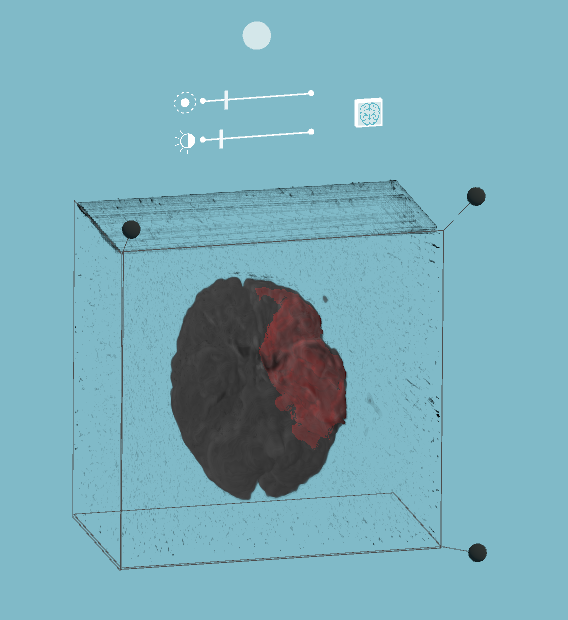
\includegraphics[width=0.5\linewidth]{images/mARt3d_2.png}
	\caption{Die 3D-Darstellung eines MRT-Datensatzes mit angezeigter Maske. Die oberen Schieberegler kontrollieren Intentsität und Gammakorrektur des Renderings. Auch hier wird der markierte Bereich durch ein Icon ein- und ausgeblendet. Jede Ebene kann durch einen Anfassungspunkt verschoben werden.}
	\label{img:mARt3d}
	\source{Eigene Darstellung}
\end{figure}
\FloatBarrier

Dieses Bedienkonzept lässt sich allerdings nicht einfach in den zweidimensionalen Raum übertragen. Da jeweils nur die ausgewählte Schicht zu sehen ist und nicht das gesamte Volumen, hat der Nutzer keine Vorstellung davon wo in dessen Innern er sich befindet. Um ihm diese zu liefern, wird die Gesamtanzahl an schichten angezeigt, sowie die wievielte gerade ausgewählt ist. 
Die Bewegung durch die Schichten erfolgt außerdem entlang der Z-Achse, die durch den zweidimensionalen Kontext allerdings wegfällt. D.h. der Wechsel zwischen den Schichten durch Anfassen und Ziehen eines Kontaktpunktes entlang dieser, wie eben beschrieben, würde nicht in das Konzept passen. 
Weiterhin sollte es dem Nutzer möglich sein die Ebene ununterbrochen zu verschieben. Bei einer Bewegung entlang der Z-Achse müsste er sehr weit vorne anfangen und ist in der Tiefe durch die Länge seines Armes beschränkt. Es wäre möglich das Interaktionselement als Schieberegler in die XY-Achse zu legen, die Bedienung ist dabei allerdings oft ungenau und könnte dazu führen, dass der Nutzer den Fokus auf den Regler legt, anstatt auf das Bild, das er auswählen will. Eine bessere Variante stellt ein Rad dar, durch dessen Rotation man zwischen den Bildern wechseln kann. Dies entspricht eher der Bedienung einer Bildschirmanwendung mittels eines Mausrads und ist dem Nutzer somit bereits bekannt. Außerdem lässt sich so eine kontinuierliche Bewegung in beide Richtungen ermöglichen. Der Nutzer muss zur Steuerung lediglich die Hand und nicht den Arm bewegen, was eine genauere Manipulation erlaubt. 
Das Rad ist dabei ähnlich einer Wählscheibe konzipiert, die der Nutzer mit einer Kreisbewegung rotiert. Verglichen mit einem Drehknopf, wie z.B. einem Lautstärkeregler, unterstützt der größere Radius mehr Kontrolle. Zudem lässt sich eine endlose Bewegung ohne Umgreifen realisieren und die Bewegung ist vom System leichter erkennbar. 
Um dem Nutzer den Eindruck von haptischen Feedback zu vermitteln und den Zustand des Elements zu verdeutlichen, wird die Berührung und Bewegung des Rades durch den Einsatz von Farbe untermalt.

%http://blog.leapmotion.com/designing-cat-explorer/

Wie in Abschnitt \ref{maske} beschrieben, wird der markierte, vom Schlaganfall betroffene Bereich innerhalb des Volumens dargestellt. Da die Maske entweder angezeigt wird oder nicht, kann der Nutzer die gewünschte Darstellung erreichen, indem er einen Schalter bedient, der zwischen den beiden Zuständen wechselt. Dies ist in \textbf{U11} gefordert.

Zur besseren Sichtbarkeit bestimmter Bereiche fordert Anforderung \textbf{U14}, dass die Helligkeit und der Kontrast der MRT-Bilder einstellbar sind. Dies ist über einen Schieberegler steuerbar, der sich oberhalb der Darstellung befindet. 
Die Manipulation von Helligkeit und Kontrast wird dabei als Gammakorrektur im Shader implementiert. Der von Nutzer bestimmte Gammawert wird dazu als Exponent zur Bildfarbe genommen. 
In der 3D-Darstellung wird außerdem ein weiterer Schieberegler angezeigt, über den der Nutzer bestimmen kann, wie intensiv Voxel dargestellt werden sollen. Diese Intensität beeinflusst die Opazität der Voxel. Ist ein hoher Wert eingestellt, werden die äußeren und damit dunkleren Voxel mit geringer Opazität dargestellt, sodass sie die weiter innen liegenden Voxel verdecken. Eine niedrige Intensität hat zur Folge, dass die äußeren Werte ausgeblendet werden, sodass die inneren Strukturen deutlicher zu erkennen sind. Auf diese Weise kann der Nutzer die Umgebung des Gehirns ausblenden und nur das Organ selbst darstellen.
Die Bedienoberfläche zur Manipulation der 2D-MRT-Daten ist in Abbildung \ref{img:mARt2d} zu sehen.

Obwohl nicht in den Anforderungen beschrieben, würde die Manipulation des gekennzeichneten Bereichs mit denselben Optionen dem Nutzer helfen die Darstellung seinen Ansprüchen anzupassen. Dies kann ebenfalls über Schieberegler gesteuert werden. Um die Anwendung überschaubar zu halten wurde allerdings davon abgesehen.


\begin{figure}[!htb]
	\centering
	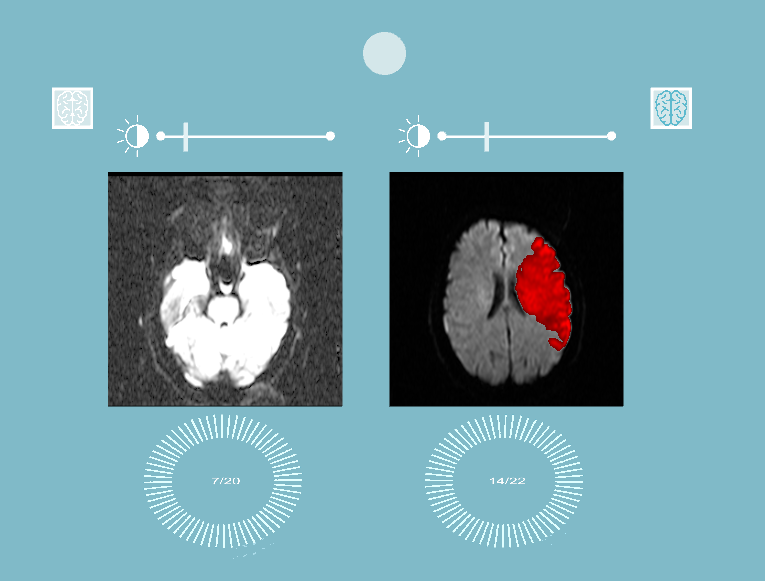
\includegraphics[width=0.7\linewidth]{images/mARt2d_2.png}
	\caption{Die zweidimensionale Darstellung von zwei MRT-Datensätzen, deren Manipulation nicht gleichgeschaltet ist. Über den oberen Schieberegler können Kontrast und Helligkeit per Gammakorrektur beeinflusst werden. Durch das Icon in der rechten Ecke kann der markierte Bereich ein- und ausgeblendet werden. Das Rad ermöglicht das Scrollen durch die Bildschichten. Die aktuelle Schicht wird in dessen Mitte angezeigt. }
	\label{img:mARt2d}
	\source{Eigene Darstellung}
\end{figure}
\FloatBarrier

% Zoom
Zu den geforderten Interaktionen gehört mit \textbf{U15} auch die Vergrößerung von Bildern, um dem Nutzer eine genaue Untersuchung zu erlauben. Bei der Vergrößerung handelt es sich im Grunde genommen um eine Skalierung des Bildes. Auch dies lässt sich gut mit einer direkten Handbewegung in Berührung mit der Darstellung umsetzten. Aus anderen Anwendungen sind Nutzern zwei Bedienmöglichkeiten dieser Funktionalität bekannt. Bei Bildschirmanwendungen wird oft das Mausrad zum Zoomen verwendet. Allerdings werden Räder bereits für andere Aktionen verwendet und ein mehrdeutiger Einsatz könnte zu Verwirrung führen. Von der Bedienung von Touchdisplays sind Nutzer weiterhin daran gewöhnt zu zoomen, indem sie den Bildschirm mit Daumen und Zeigefinger berühren und die Finger dann aufeinander zu oder voneinander weg bewegen. Diese Bewegung lässt sich gut in die Anwendung übertragen. Um ein eindeutigeres Ergebnis zu erhalten und dem Nutzer mehr Kontrolle zu geben werden statt zwei Fingern allerdings die beiden Hände verwendet. Wird das Bild von beiden Händen mit Daumen und Zeigefinder gegriffen kann es durch die Bewegung der Hände zueinander skaliert werden.

Um zu verhindern, dass zwei Darstellungen sich durch die Skalierung unterscheiden und die Anwendung überschaubar zu halten, ist eine Vergrößerung nur möglich, wenn ein einzelner Datensatz angezeigt wird. 
Das Vergrößern ist dabei als temporäre Manipulation konzipiert. Wenn der Nutzer einen zweiten Datensatz zur Visualisierung auswählt, wird der erste auf seine ursprüngliche Größe zurück gesetzt. Die Skalierung wird auch nicht in die andere Szene übertragen, wenn der Nutzer zwischen 2D und 3D wechselt. Dies kann dem Nutzer auch als bewusstes Zurücksetzten dienen, falls er die Skalierung beispielsweise versehentlich übertrieben hat.

% Verschieben
Die User Story \textbf{U16} fordert die Möglichkeit die Darstellung verschieben zu können. %Ersteres beschreibt dabei die Verschiebung im Raum, zweiteres eine Verschiebung der Darstellung. 
%Die beiden interaktionen wurden zu einer zusammen gefasst. 
Über den Bedienelementen einer Ansicht wird jeweils ein greifbares Objekt platziert. Durch das Greifen, Ziehen und Loslassen des Objektes kann der Nutzer die gesamte Darstellung verschieben. %Damit ist die Positionierung im Raum abgedeckt. 
Vergrößert der Nutzer eine Darstellung kann er dieselbe Verschiebung nutzen, um sich darin zu orientieren. 
%Zwar ist die Verschiebung auf die Armreichweite des Nutzers beschränkt, sofern er sich nicht im Raum bewegt, aber eine übermäßige Skalierung ist generell sowieso nicht erstrebenswert.
Um die Darstellung der Position des Nutzers weiterhin anpassen zu können, kann diese gedreht werden. Dazu dient ein weiteres Bedienelement, welches sich vor der Darstellung befindet. Um die Anwendung übersichtlich zu gestalten, erscheint dieses nur, wenn der Nutzer das erste Element ergriffen hat und somit seine Absicht demonstriert, die Darstellung zu bewegen. 
Sowohl Position als auch Rotation der Ansicht werden beim Szenariowechsel übernommen.
Die Bedienelemente zur Positionierung und Drehung der Ansicht sind in Abbildung \ref{img:3dPos} dargestellt. 

\begin{figure}[!htb]
	\centering
	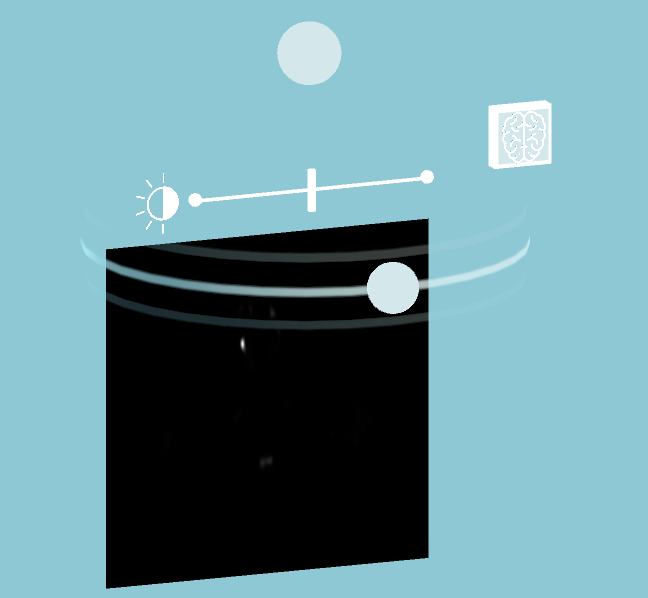
\includegraphics[width=0.5\linewidth]{images/mARt_turn.png}
	\caption{Die zweidimensionale Darstellung mit den beiden Bedienelementen zur Positionierung (oben) und Drehung (mitte).}
	\label{img:3dPos}
	\source{Eigene Darstellung}
\end{figure}
\FloatBarrier

Die Darstellung der MRT-Daten soll weiterhin nach \textbf{U17} die ihr gegebene Position behalten, sodass der Nutzer um sie herum gehen und von allen Seiten betrachten kann, oder an einem bestimmten Standpunkt verankern kann. Dies wäre vor allem in einem Multi-Nutzer-Szenario nützlich, in dem mehrere Nutzer gleichzeitig die Daten betrachten.
Die Bedienweise sollte sich durch diese Funktionalität nicht ändern. Zu deren Umsetzung gibt es verschiedene Ansätze, die in Abschnitt \ref{anchor} erläutert werden.

%Drehen
Entsprechend Anforderung \textbf{U13} soll die volumetrische Darstellung der MRT-Daten gedreht werden können. 
Die Drehung erfolgt dabei durch das Greifen des Volumens und Bewegen der Hand. Diese direkte Manipulation ist sehr intuitiv, wenn auch nicht unbedingt genau. Eine gradgenaue Drehung würde bei der Verwendung von mARt allerdings keinen erkennbaren Vorteil bringen. 
Wird das Volumen gedreht, drehen sich die Kontrollpunkte zum Verschieben der Bildebenen mit, um die lokale Verbindung zwischen diesen und der Ebene, die sie manipulieren zu erhalten. Würden sie sich nicht bewegen, wäre es schwer vorauszusehen, welcher Kontrollpunkt welche Ebene beeinflusst. 
Die UI wird von der Rotation allerdings nicht beeinflusst, da ihre Bedienung nur erschwert würde, wenn sie nicht annähernd orthogonal zur Blickrichtung des Nutzer verlaufen würde. 
Ebenso wie die Skalierung, ist die Rotation eine temporäre Manipulation, die beim Szenenwechsel zurückgesetzt wird.

Die User Story \textbf{U04} erfordert es weiterhin, dass Bilder im direkten Vergleich nebeneinander betrachtet werden können. Dies gilt sowohl für die zwei- als auch dreidimensionale Darstellung der Daten. Die User Stories \textbf{U05} und \textbf{U06} erfordern außerdem eine Möglichkeit für den Nutzer aus den vorhandenen Daten einzelne auszuwählen, die angezeigt werden sollen, sowie die Daten jeweils gleichzeitig oder einzeln zu manipulieren. 
Die Auswahl der Datensätze, sowie die Wahl ob diese synchron manipuliert werden sollen oder nicht, sind beide nicht Teil der direkten Manipulation des Bildes. Sie müssen deshalb nicht in dessen unmittelbarem Umfeld stehen und der Nutzer kann während dessen Bedienung auch auf diese den Fokus setzen.
 
Die Bedienung der entsprechenden Interaktionselemente sollte trotzdem intuitiv und schnell umzusetzen sein. Da die Option der Synchronizität abhängig ist von der Tatsache, ob ein oder mehrere Datensätze angezeigt werden, stehen die beiden Aktionen in Verbindung zu einander und werden deshalb in einem Menü vereint, das für beide Darstellungen verwendet wird. Dieses wird an der linken Hand des Nutzers verankert. Auf diese Weise kann es immer schnell erreicht werden und wird nicht unbeabsichtigt aus den Augen verloren. Gleichzeitig fördert es die Immersion der Anwendung, da der Nutzer quasi Teil von ihr wird. Ein Effekt, der in einer Bildschirmanwendung nicht umsetzbar wäre. 

Damit das Menü nicht während der Verarbeitung der Bilder stört, wird es nur dann eingeblendet, wenn der Nutzer seine Handfläche Richtung Kamera dreht und diese somit ansieht. Das \textit{Leap Motion} SDK bietet eine Beispielszene, die dies umsetzt.
Eine besondere Herausforderung bei der Konzeption des Menüs ist es, dieses möglichst einfach und platzsparend zu halten. Der Bereich der \textit{Leap Motion} Kamera, in dem die Hände erkannt werden ist beschränkt. Deshalb kann es bei einer Interaktionsfläche, die viel Raum davon einnimmt dazu kommen, dass der Nutzer versehentlich Knöpfe betätigt. 
Um den Umfang des Menüs in benutzbaren Dimensionen zu halten, wurde es auf drei Knöpfe reduziert. 
Die Liste der verfügbaren Datensätze kann darin allerdings nicht untergebracht werden. Deshalb kann sie bei Bedarf über einen der Knöpfe ausgeklappt werden. 
Indem der Nutzer einen Datensatz auswählt, wird dieser auf der Bildfläche angezeigt. Die Auswahl ist auf zwei Datensätze beschränkt. Zu viele gleichzeitig dargestellte Bilder würden unübersichtlich wirken und die Motivation hinter der User Story ist der direkte Vergleich zweier Bilder. Außerdem stellen mehr Bilder auch mehr Möglichkeiten dar diese in verschiedenen Kombinationen zu manipulieren. Dies hätte die Anwendung unnötig verkompliziert. 
Stattdessen wird die Synchronisierung der Manipulation über einen weiteren Knopf im Handmenü gesteuert. Dieser ist nur aktiv, wenn tatsächlich zwei Bilder angezeigt werden. Dann funktioniert er als Schalter. Indem der Nutzer ihn betätigt wird jeweils nur eine Benutzeroberfläche über beiden Bildern angezeigt oder sie wird dupliziert und für jede Darstellung eingeblendet. 
 
Schließlich kann der Nutzer durch das Handmenü auch zwischen der zwei- und dreidimensionalen Darstellung wechseln, wie es in \textbf{U09} beschrieben ist. Auf dem dafür zuständigen Button wird jeweils das Szenario angezeigt, in das gewechselt wird.
Laut \textbf{U10} sollen beim Wechsel die Manipulationen und Einstellungen möglichst erhalten bleiben. D.h. wenn in 2D zwei Datensätze angezeigt werden, einer mit und einer ohne Maske, sollte das nach dem Wechsel zu 3D ebenfalls so sein. 
Bis auf die genannten Ausnahmen werden die Einstellungen, die in einer Ansicht getätigt werden in die andere übernommen. Handelt es sich um Werte, die nur in einer der beiden Szenarios vorhanden sind, wie die Position der zusätzlichen Ebenen der 3D-Darstellung, werden diese ebenfalls gespeichert.
In Abbildung \ref{img:handUI} ist das ausgeklappte Menü, an der linken Hand dargestellt.

\begin{figure}[!htb]
	\centering
	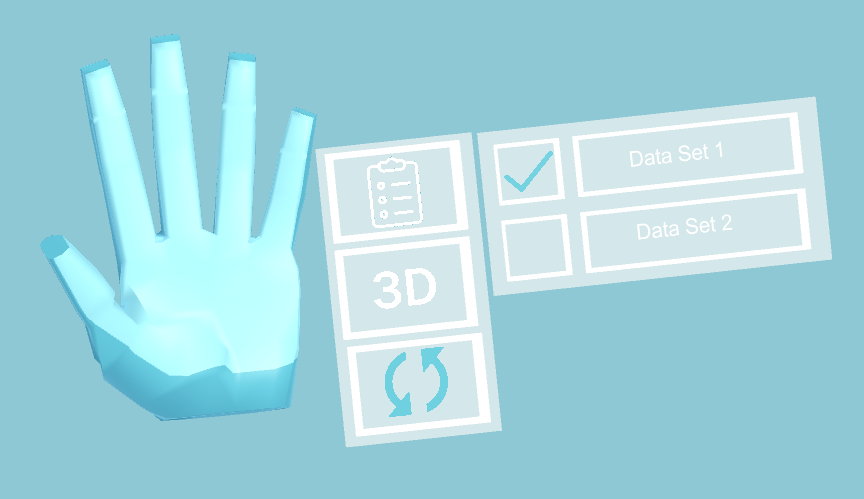
\includegraphics[width=0.7\linewidth]{images/handUI_2.png}
	\caption{Das ausklappbare Handmenü, das erscheint, wenn der Nutzer seine Handfläche zur Kamera dreht. Über die Knöpfe kann der Nutzer die angezeigten Datensätze auswählen (oben und Liste), zwischen 2D- und 3D-Darstellung wechseln (mitte) und die angezeigten Datensätze gleichschalten (unten). }
	\label{img:handUI}
	\source{Eigene Darstellung}
\end{figure}
\FloatBarrier

\subsection{Interaktion AR}

Die Interaktionen bleiben in der AR- und VR-Version der Anwendung gleich, da für beide die \textit{Leap Motion} zur Steuerung verwendet wird.
Im Gegensatz zum Einsatz in VR sind allerdings die realen Hände des Nutzers für diesen sichtbar, während er die Anwendung in AR bedient. Da durch die \textit{Leap Motion} die Hände zusätzlich virtuell simuliert werden, sieht der Nutzer vier Hände, was zuerst verwirrend wirken kann. 
Die Leap-Controller-Hände für den Nutzer unsichtbar zu machen, wäre zwar möglich, ist allerdings nicht die beste Vorgehensweise. Obwohl die \textit{Leap Motion} die Hände und Handbewegungen zuverlässig nachempfindet, verhalten die virtuellen Hände sich nicht ganz deckungsgleich zu den realen. Dies hängt auch damit zusammen, dass die \textit{Leap Motion} Kamera sich ein Stück vor oder über den Augen des Nutzers befindet, da sie am HMD befestigt ist. Dieses Problem wird auch in Abschnitt \ref{kombination} beschrieben.
Die Abweichungen der Simulation sind in einer VR-Anwendung deutlich weniger auffällig. Durch die Immersion der virtuellen Welt und dem Fehlen eines direkten Vergleichs mit der realen, entsteht beim Nutzer die Illusion, dass die virtuellen Hände sich genau dort befinden, wo er seine echten Hände vermutet. Dies ist durch die Dominanz der visuellen Wahrnehmung begründet, wie sie z.B. \cite{Azmandian16} beschreiben.

In AR entfällt diese Illusion. Da die beiden Handpaare aber nicht deckungsgleich sind, kann es dazu kommen, dass ein virtueller Finger einen Knopf trifft, während es ein realer nicht tut oder umgekehrt. Wenn der Nutzer die virtuelle Hand nicht sieht, würde dies den Eindruck von fehlerhaftem Verhalten hervorrufen. 
Aus diesem Grund werden die Leap-Controller-Hände auch in der AR-Anwendung angezeigt. Allerdings werden sie leicht transparent dargestellt, um dem Nutzer zu erlauben auch die dahinter liegende Umgebung wahrzunehmen. 
In Abbildung \ref{img:arHands} sind die Hände innerhalb der Anwendung abgebildet.

\begin{figure}[!htb]
	\centering
	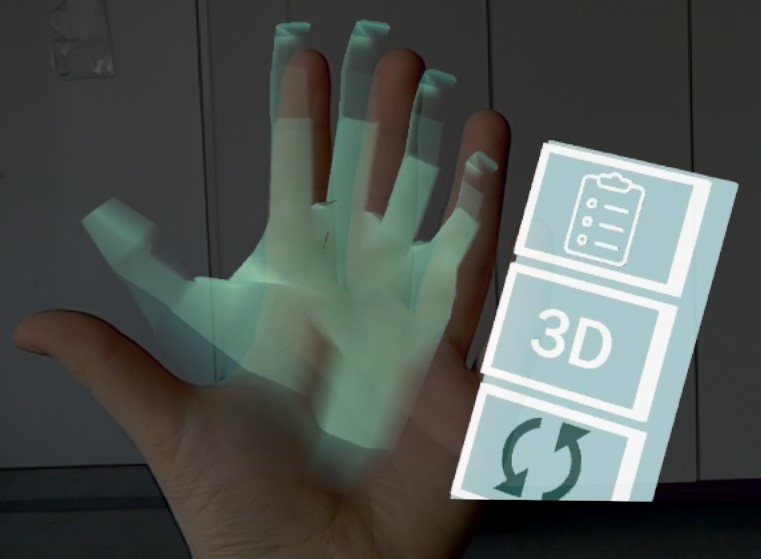
\includegraphics[width=0.5\linewidth]{images/AR_hand.jpg}
	\caption{Aufnahme aus der \textit{HoloLens}, die die augmentierte Hand des Nutzers zeigt.}
	\label{img:handUI}
	\source{Eigene Darstellung}
\end{figure}
\FloatBarrier


\section{Unterstützung von Dateiformaten} 

In den im Kapitel \ref{anforderung} beschriebenen Anforderungen ist durch \textbf{U19} und \textbf{U20} beschrieben, dass mARt gängige Dateiformate zur Speicherung von medizinischen Bilddaten, insbesondere NIfTI und DICOM unterstützt. Beide Formate wurden im Kapitel \ref{grundlagen} beschrieben. 
Um die MRT-Bilder verarbeiten und darstellen zu können, muss eine Parser oder Converter in das Programm eingebunden werden. 
Der Nutzer könnte dann über eine Schnittstelle die Daten direkt in die Anwendung laden, wo sie umgewandelt und angezeigt würden. 

In einer realen Arbeitsumgebung ist diese Funktionalität mehr als sinnvoll. Wie allerdings in Kapitel \ref{anforderung} beschrieben, soll es sich bei mARt in erster Linie um einen Prototyp handeln.
Der Fokus soll dabei auf der Darstellung der Daten und der Interaktion mit ihnen liegen. Da der zur Entwicklung und zum Testen zur Verfügung stehende Datensatz gering ist, ist die Nützlichkeit in diesem Szenario nicht gegeben. Der benötigte Zeitaufwand zur Implementierung wird somit nicht durch einen Mehrwert gerechtfertigt.
Weiterhin kann so die Komplexität und der Umfang der Anwendung gering gehalten werden, was es dem Nutzer erlaubt sich auf die Kernfunktionen zu konzentrieren. 

Durch den eingeschränkten verfügbaren Datensatz, konnte auch \textbf{U18}, nicht umgesetzt werden, da jeder Datensatz nur in einer Sequenz zur Verfügung steht.

Trotzdem können mehrere Datensätze in mARt dargestellt werden. Diese werden durch Verwendung von externer Bildsoftware manuell in PNG-Dateien umgewandelt und in die Anwendung integriert, bevor diese gebaut wird. 
Obwohl dieser manuelle Vorgang umständlich ist, ist er für den Zweck der Anwendung und den Umfang dieser Arbeit ausreichend.

% Implementierung

\chapter{Implementierung}
\label{implementierung}

Nachdem das Konzept der Anwendung beschrieben wurde, wird in den folgenden Abschnitten auf die Implementierung von mARt eingegangen. 

\section{Aufbau Struktur des Projektes}

Wie im Kapitel \ref{konzept} erläutert wurde, stellt mARt jeweils eine zwei- und dreidimensionale Darstellung der MRT-Daten zur Verfügung, zwischen denen gewechselt werden kann. Auf Grund der beschriebenen Hindernisse bezüglich der Leistungsfähigkeit der \textit{HoloLens} wurde die Anwendung sowohl für die \textit{HoloLens}, als auch als VR-Anwendung implementiert. Die AR-Anwendung kann dabei nicht für die \textit{HoloLens} bereitgestellt werden. Aus diesem Grund wird die nur auf dem Gerät abgespielt. In beiden Fällen handelt es sich im Kern um die selbe Anwendung, d.h. die Software sollte für beide Gräte entwickelt werden. 
Sowohl für die Entwicklung von VR- als auch AR-Anwendungen werden im Allgemeinen Spiele-Engines verwendet, da sie einen Editor bieten, um interaktive 3D-Anwendungen zu erzeugen, die in Echtzeit funktionieren. 
Zur Implementierung von mARt wurde \textit{Unity} von \cite{unity} verwendet. Die Engine gehört zu den meist genutzten auf dem Markt. Laut \cite{unityRelations} selbst, werden 60\% von AR/VR Inhalten mit \textit{Unity} entwickelt. Weiterhin ermöglicht \textit{Unity} die Entwicklung von Software für die meisten Plattformen. \textit{Unity} bietet viele nützliche Funktionen zur Entwicklung von interaktiven Anwendungen und wird außerdem von einer großen  Gemeinschaft genutzt, sodass neben einer detaillierten Dokumentation auch über Foren und Webartikel hilfreiche Informationen zur Entwicklung zur Verfügung stehen.

\textit{Microsoft} empfiehlt weiterhin \textit{Unity} zur Entwicklung für \textit{HoloLens}-Software zu nutzen \cite{unityHololens} und bietet mit \textit{Mixed Reality Toolkit} (MRTK) von \cite{holoToolkit} ein Framework, das \textit{HoloLens}-Funktionen innerhalb von \textit{Unity} zur Verfügung stellt.
\textit{Unity} verwendet C\# als Skriptsprache. Die Engine selbst ist allerdings in C++ geschrieben, wodurch effiziente Berechnungen zur Laufzeit ermöglicht werden.
\todo{Referenzen?}
%Wieso?

mARt wurde in \textit{Unity} entwickelt und sollte dann sowohl für die \textit{HoloLens} und als VR-Anwendung gebaut werden. Die Anwendung konnte allerdings nicht für die \textit{HoloLens} bereitgestellt werden. Diese Problematik wird in Abschnitt \ref{kombination} erläutert.
Um die \textit{Unity}-Anwendung auf dem VR-System abzuspielen, wird die \textit{SteamVR}-Software von \cite{steam} in das Projekt integriert. Um die Anwendung starten zu können muss sie auf dem jeweiligen Computer installiert sein.

\subsection{\textit{Unity} Projekt}

\textit{Unity} Projekte basieren auf 3D-Szenen. Innerhalb einer Szene können GameObjects platziert werden. Dabei kann es sich z.B. um 3D-Modelle handeln. Ein GameObject besitzt verschiedene Components, die dessen Eigenschaften und Verhalten bestimmen. Viele Funktionen und Eigenschaften werden von bereits in der Engine vorhandenen Components realisiert. Sogenannte Rigidbodys verleihen einem Objekt beispielsweise physikalische Eigenschaften, die von der Engine berechnet werden. Components können auch Skripte sein, die der Entwickler selbst verfasst hat. Über diese Skripte wird die Spiellogik und die Funktionalität der Anwendung definiert. 

Da mARt sich in die beiden Szenarien einer zwei- und dreidimensionalen Darstellung unterteilen lässt existiert für jedes Szenario eine Szene.
Viele der Funktionen sind allerdings ähnlich oder gleich, weshalb manche Skripte in beiden Szenen verwendet werden. 
Zusätzlich zu den beiden Szenen existiert eine Startszene Main/Preload.unity, in der ein GameObject namens appState liegt, über das bestimmt werden kann welche Szene zuerst geladen werden soll. In diesem Objekt werden auch die Zustände der Szenen gespeichert und so Manipulationen übertragen.
Die Szenen für die 2D-Darstellung sind 2DUI/main\_2D.unity und 2DUI/main\_2D\_AR.unity. Die für die 3D-Darstellung 3DUI/main\_3D.unity und 3DUI/main\_3D\_AR.unity.



\section{Shader in Unity}

Wie in Kapitel \ref{konzept} beschrieben wurde, wird das Volume Rendering der MRT-Daten in einem Shaders umgesetzt. An dieser Stelle soll ein Überblick über die Funktionsweise und den Aufbau von \textit{Unity}-Shadern gegeben werden. Aufbau und Funktionsweise sind in der \textit{Unity}-Dokumentation von \cite{unityDoku} beschrieben.

Wie ein Objekt in einer Szene gerendert wird hängt in \textit{Unity} davon ab, welches Material diesem zugewiesen ist. Das Material fungiert dabei als Behälter für sämtliche Parameter, die das Aussehen des Objektes beeinflussen, wie z.B. die Textur oder Farbe. Welche Parameter das Material besitzt und wie diese miteinander verrechnet werden bestimmt der Shader des Materials. Innerhalb des Shaders wird in Abhängigkeit zu den diesem übergebenen Werten die Farbe für jeden Pixel errechnet. 
% https://docs.unity3d.com/Manual/Shaders.html

Shader in \textit{Unity} sind in der \textit{Unity} eigenen Shader-Sprache Shader Lab geschrieben. Im Shader ist definiert welche Eigenschaften dieser besitzt und welche Sub- und Fallback-Shader er verwendet.
Die Eigenschaften sind die eben genannten Parameter, deren Werte dann über das Material gesetzt werden. Hier werden deren Namen, Typen, ihr Wertebereich sowie ihre Standardwerte definiert. 

Schließlich werden im Shader auch sogenannte Subshader definiert, die den eigentlichen Shader-Code enthalten.
Ein Shader kann mehrere Subshader enthalten für den Fall, dass einer der Shader von einem Gerät nicht unterstützt wird. Wird keiner unterstützt wird der Fallback-Shader verwendet. 
Neben dem Shader-Code besitzt ein Subshader Tags, die bestimmen wann und wie ein Shader von der Rendering-Engine gerendert werden soll. Dies kann sich beispielsweise auf die Reihenfolge beziehen, in der Objekte gerendert werden oder ob ein Objekt Schatten werfen soll. 
Nach den Tags folgt die Definition eines Pass. Als Render Pass wird der gesamte Prozess bezeichnet, der durchlaufen wird, um einen Pixel zu rendern. Angefangen bei der Berechnung einzelner Vertices eines Meshes über den Vertex-Shader bis zum Fragment-Shader. D.h. im Pass werden in verschiedenen Methoden die tatsächlichen Berechnungen beschrieben, die zum Aussehen jedes Pixels führen. 
Auch ein Pass kann zunächst wieder Tags enthalten, die bestimmen wann oder wie oft ein Pass durchlaufen werden soll. 
% Render setup ????
Dann folgt der Abschnitt, der den Shader-Code enthält. Dieser ist in Cg (C for Graphics)
\todo{REFERENZ} geschrieben, einer Shading-Sprache, die syntaktisch stark HLSL (High-Level Shading Language) ähnelt. 
Abhängig davon um welche Art von Shader es sich handelt, werden hier die notwendigen Funktionen implementiert. \textit{Unity} besitzt sogenannte Surface-Shader,  vereinfachte Shader, für die kein Beleuchtungsmodell implementiert werden muss. Andererseits können auch Unlit-Shader implementiert werden, in deren Pass Vertex- und Fragment-Shader definiert sind. 
Das Volume Rendering der MRT-Daten erfolgt durch einen Unlit-Shader. Auf die genaue Implementierung wird im Folgenden eingegangen. 

% https://docs.unity3d.com/Manual/SL-Shader.html
\todo{ P
REFERNZEN
}
\section{Grundlage der Implementierung}

Die in Kapitel \ref{anforderung} beschriebenen Anforderungen repräsentieren den Umfang der zu implementierenden Anwendung. 
Neben der Umsetzung der Anwendungslogik stellt vor allem die Implementierung der 3D-Darstellung durch Volume Raycasting einen hohen Aufwand dar. Um diesen in einem realisierbaren Rahmen zu halten, wurde ein bereits existierendes Programm als Basis für die zuletzt genannte Funktionalität verwendet.
Wie in Kapitel \ref{grundlagen} beschrieben wurde, gibt es bereits viele Implementierungen von Volume Raycasting zur Visualisierung von medizinischem Bildmaterial. 
Die dort genannten Unity-spezifischen Lösungen sind allerdings kostenpflichtig und/oder ihre Codebasis ist nicht einsehbar. Es wäre allerdings von Vorteil die Kontrolle über die Implementierung der 3D-Darstellung zu haben, um so die Möglichkeit zu haben, sie den Anforderungen entsprechend anpassen zu können.
Aus diesem Grund wurde die Open-Source-Implementierung von \cite{volumeRenderingGit} als Grundlage für die 3D-Darstellung verwendet, die unter der MIT-Lizenz steht.
Diese wurde erweitert, um die Anforderungen an mARt zu erfüllen. 
Im Rahmen der Arbeit wurden folgende Bestandteile implementiert:

\begin{itemize}
\item Erweiterung des Shaders (Maske, Beleuchtung)
\item Umwandlung von Bilddaten in 3D-Texturen und der Berechnung ihrer Gradienten
\item Anpassung der Bedienelemente an 3D-Szene
\item Anwendungslogik
\end{itemize}
Der fremde Code ist im Projekt gekennzeichnet.

\section{Volume Rendering}

Wie in Kapitel \ref{konzept} beschrieben wurde, wurde die 3D-Darstellung des Gehirns mit Hilfe von Volume Raycasting umgesetzt. 
Im Abschnitt \ref{rayCasting} wurde der theoretische Vorgang dieser Technik beschrieben. Dieser Abschnitt fokussiert sich auf die Implementierung der einzelnen Schritte.

Die volumetrische Darstellung des Gehirns wird mit drei Skripten erzeugt. Zuerst wird in VolumeRendering/Scripts/VolumeRendering.cs das Mesh des Würfeln generiert. Hier werden auch die Parameter aktualisiert, die für das Rendering relevant sind, wie z.B. die 3D-Textur oder Farbe, sowie die Parameter, die durch die Nutzerschnittstelle manipuliert werden können. 
Die Parameter werden an den Shader VolumeRendering/Shader/VolumeRendering\_Diffuse\_Mask.shader übergeben, in dem das Rendering definiert ist. Der Cg-Code, der den Vertex- und Fragment-Shader implementiert ist dabei in ein eigenes Skript VolumeRendering/Shader/VolumeRendering\_Diffuse\_Mask.cginc ausgelagert.

\subsection{Volume Raycasting}
\label{3dImplementierung}
Im Fragment-Shader des VolumeRendering/Shader/Volume\_Diffuse\_Mask.sh Shaders wird zunächst ein Strahl definiert, der von dem aktuell betrachteten Vertex aus von der Kameraposition in die Welt geschossen wird. In einem selbst definierten struct werden die maximalen und minimalen Werte definiert, aus denen sich die Eckpunkte des dargestellten Quaders zusammensetzten. Anschließend wird geprüft, ob der Strahl den Würfel schneidet. 

%-----------Intersect-----------
%Dies geschieht indem zuerst die Inverse der Strahlrichtung ermittelt wird. Die Inverse eines Vektors $v$ ist $v^-1$ und da $v^-x=\frac1}{v^x}$, ergibt sich die Inverse des Richtungsvektors des Strahls indem $1$ durch die dividiert wird.
% AABB, axis aligend etc? intersection formula REFERENZ
Um die Schnittpunkte des Strahls zu ermitteln nimmt man an, dass die sechs Seiten des Würfels auf jeweils sechs Ebenen liegen, wobei davon zwei immer parallel sind. Zuerst werden alle Schnittpunkte des Strahls mit diesen Ebenen berechnet und dann geprüft, ob die Schnittpunkte innerhalb des Würfels liegen.
Der Würfel wird durch zwei Eckpunkte beschrieben. Da der Würfel Koordinaten von -0,5 bis 0,5 hat können wir hierfür die jeweils kleinsten und größten Koordinaten nutzen. 
Die Schnittpunkte des Strahls, mit den X-, Y- und Z-Ebenen ergeben sich durch das Umstellen der Formel, die einen Strahl beschreibt:

\begin{align}
p=r_{Ursprung}+t*r_{Richtung}
\end{align}

$r_{Ursprung}$ ist dabei der Ursprung des Strahls und $r_{Richtung}$ seine Richtung. $p$ ist ein Punkt auf dem Strahl und $t$ ein Parameter, der bestimmt wie weit der Punkt vom Ursprung entfernt ist.

Um die Schnittpunkte mit den Ebenen zu erhalten wird die Formel nach $t$ umgestellt:

\begin{align}
t=(p-r_{Ursprung})/r_{Richtung}
\end{align}

Für $p$ werden jeweils die beiden Eckpunkte des Würfels, die jeweils auf drei der Würfelebenen liegen, eingesetzt.
Dadurch sind insgesamt sechs $t$s und damit sechs Schnittpunkte mit den Ebenen bekannt. Zwei für jedes Ebenenpaar. Die Entfernungen werden in den zwei dreidimensionalen Vektoren $t_{unten}$ und $t_{oben}$ gespeichert. Durch den Vergleich der t-Vektoren wird festgelegt, welcher Eckpunkt und damit welche zweier paralleler Ebenen weiter vorne liegt. 
% Was wenn Strahl parallel zur Ebene ist??
Jetzt muss bestimmt werden, ob diese Schnittpunkte sich innerhalb des Würfels befinden.
Dazu werden jeweils die x-, y- und z-Werte der t-Vektoren untereinander verglichen. Für das $t$ der näher gelegenen Ebene wird der maximale, für den weiter entfernten der minimale Wert bestimmt. Ist der Wert des näheren $t$s größer als der des entfernten, schneidet der Strahl den Würfel nicht. Andersherum tut er es.
Das Verhältnis der Schnittpunkte zueinander und wie dieses durch den Verlauf des Strahls bestimmt wird ist in Abbildung \ref{img:rayBoxHit} dargestellt.

\begin{figure}[!htb]
	\centering
	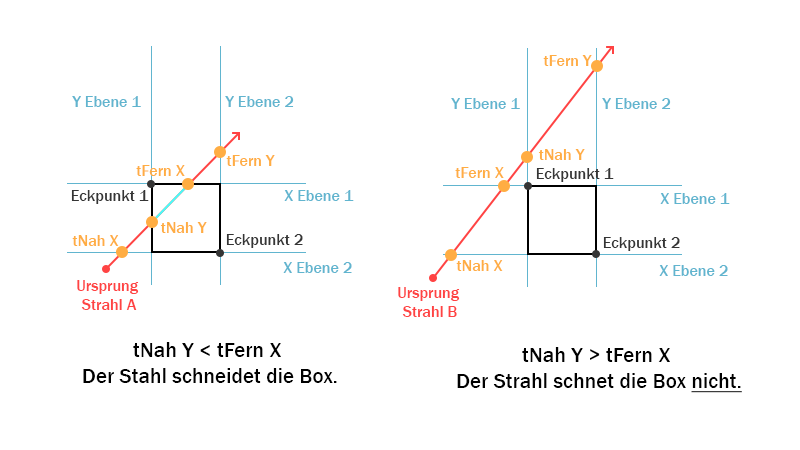
\includegraphics[width=0.9\linewidth]{images/rayBox.png}
	\caption{Zweidimensionale Darstellung, wie ein Strahl durch einen Würfel (links) und daran vorbei (rechts) verläuft. Die Schnittpunkte des Strahls (gelb) mit den Würfelebenen (blau) sind eingezeichnet. Der Vergleich derer Abstände zum Ursprung des Strahls (rot) zeigt, ob der Strahl den Würfel schneidet oder nicht.}
	\label{img:rayBoxHit}
	\source{Eigene Darstellung}
\end{figure}
\FloatBarrier

%----------------------------------------
Die beiden t-Werte werden als $t_{nah}$ und $t_{fern}$ gespeichert.
Mit dem Ursprung des Strahls und $t_{fern}$ werden Anfang, Ende und die Länge des Strahls berechnet. Mit Hilfe der Länge kann ermittelt werden um wie weit pro Iteration am Strahl entlang gegangen werden soll. Dadurch wird der Strahl nur bis zu seinem Austritt aus dem Würfel abgetastet. 

In einer for-Schleife wird jeder Strahl nun abgetastet. In jeder Iteration wird jeweils ein Punkt betrachtet. Der Punkt verschiebt sich entlang des Strahls um die zuvor berechnete Distanz.
Für jeden Punkt werden zuerst die Texturkoordinaten berechnet.
Für die Koordinaten werden dann die jeweiliges Isowerte aus der 3D-Textur gelesen, die zuvor mit den MRT-Bildern befüllt wurde.

%---------------SAMPLE VOLUME-------------
Hierbei werden lediglich die Texturkoordinaten als Indices für die Textur verwendet. 
Der Isowert ist dabei im Alphakanal der Textur gespeichert. Da es sich nicht um eine Farbe sondern nur einen Grauwert handelt, können die anderen Farbkanäle der Textur mit dem Gradienten des jeweiligen Pixels befüllt werden. Darauf wird im Abschnitt \ref{gradienten} genauer eingegangen.

Der Isowert wird außerdem noch mit der Intensität multipliziert, die der Nutzer beeinflussen kann.
An dieser Stelle wird aber auch geprüft, ob der betreffende Punkt überhaupt zu sehen ist oder aufgrund der verschiebbaren Schichten nicht sichtbar sein sollte. 
Dazu wird zuerst der aktuell betrachtete Punkt mit der Rotationsmatrix des Volumens multipliziert.
Der Punkt wird dann mit den von Nutzer eingestellten minimalen und maximalen X-, Y-, und Z-Werten der verschiebbaren Schicht verglichen, die den sichtbaren Bereich definieren. Das Ergebnis des Vergleichs wird dabei in einer Variable gespeichert. Ist der Punkt kleiner als das Minimum oder größer als das Maximum wird 0 gespeichert, ansonsten 1. 
Die beiden Werte werden anschließend mit dem Isowert multipliziert. Ist einer der Werte 0, ist auch der ermittelte Isowert 0, was im Alphakanal totale Transparenz bedeutet. 
Das Ergebnis dieser Berechnung wird zunächst jedem Farbkanal zugewiesen.
%-----------------------------------------

An dieser Stelle wird über die Transferfunktion der entsprechende Alphawert aus der zugehörigen Textur gelesen. Dazu wird der Isowert als Index verwendet. Die Funktionsweise und Implementierung der Transferfunktion wird in der Sektion \ref{transfer} beschrieben.
% Bezug Transferfunktion!
Die Transferfunktion wird nur abgerufen, wenn der Isowert nicht 0 ist, da sonst die Transparenz überschrieben würde.
% Tranferfunktion bei index 0 auf 0000 setzen??
Ist die Farbe bekannt, wir der betrachtete Voxel illuminiert. Dies ist in der Sektion \ref{illumination} beschrieben. 
Der Alphawert der so erhaltenen Farbe wird noch einmal halbiert, um die Darstellung semi-transparent erscheinen zu lassen.
% WARUM
Schließlich wird der erhaltene Farbwert mit den vorhergehenden verrechnet. Die Komposition erfolgt dabei von vorne nach hinten, da der Strahl in dieser Richtung abgetastet wird, nach der in Kapitel \ref{grundlagen} beschriebenen Formel.
% Referenz GPU Gems
Wenn diese Farbe einen zuvor definierten Schwellenwert überschreitet wird die Schleife abgebrochen. 
Die Farbe wird schließlich noch auf einen Wert zwischen 0 und 1 festgesetzt und mit der Farbe der Maske verrechnet, die auf dem selben Weg aber ohne die Verwendung einer Transfertextur bestimmt wurde.

\subsection{Transferfunktion}
\label{transfer}

Wie beschrieben, wird die Transfertextur im Shader ausgelesen. Vorher wird sie von dem Skript 3DUI/Scripts/CreateTransferColorTexture.cs erzeugt, welches beim Ausführen der Szene 3DUI/Scenes/Load3DTexture.unity ausgeführt wird.
Um eine Transfertextur zu erzeugen, werden zunächst zwei Key-Value-Listen definiert, in denen über Kontrollpunkte bestimmte Isowerte einem Farb- oder Opazitätwert zugewiesen werden. Mit Hilfe einer Schleife wird dann eine 2D-Textur mit den Dimensionen 256 und 1 erstellt. Dabei wird für jeden X-Wert der Textur geprüft, ob er größer oder gleich dem Isowert des betrachteten Kontrollpunktes ist. Ist dies der Fall, wird der Pixel der Textur mit dem entsprechenden Wert besetzt. Dies geschieht für alle Kontrollpunkte.
Die Textur wird dann als 2D-Textur abgespeichert. Da allein die Isowerte als Index für die Zuordnung verwendet werden, handelt es sich eigentlich um eine eindimensionale Transferfunktion. 
Allerdings werden von \textit{Unity} keine 1D-Texturen als Shader-Eigenschaften unterstützt. Da die Verwendung einer 2D-Textur aber keine Nachteile aufweist, wird stattdessen eine 2D-Textur verwendet, die eine einzige Y-Koordinate besitzt. 
Die Textur wird dann über das Material an den Shader übergeben. Wie im Abschnitt \ref{3dImplementierung} beschrieben, wird die Textur dann mit Hilfe eines Index ausgelesen.

Die Erstellung einer passenden Transfertextur ist allerdings, wie beschrieben, sehr schwierig und es konnte im Rahmen dieser Arbeit keine sinnvollen Kontrollpunkte zur Einfärbung des Volumens ermittelt werden. Aus diesem Grund wird nur der Alphawert der Transferfunktion verwendet. Auf diese Weise werden irrelevante Bildinformationen, wie Umgebungsrauschen und der Schädel ausgeblendet, wobei die Struktur des Hirninneren bestehen bleibt. 

\subsection{Beleuchtung}
\label{illumination}

Das Volumen wird mit mit dem Phong-Beleuchtungsmodell illuminiert, wodurch es mehr Plastizität erhält. Das Modell wurde bereits in Kapitel \ref{grundlagen} detailliert beschrieben. Deshalb wird an dieser Stelle nur auf die Umsetzung im Shader eingegangen.
% Referenz? warum nicht blinn?
Wie beschrieben setzt sich das Modell aus drei Komponenten zusammen: Der ambienten und der diffusen Beleuchtung, sowie der spiegelnden Reflexion. Die Komponenten werden zusammen addiert, wodurch die endgültige Farbe entsteht. 
Die Koeffizienten werden im Shader durch Farben repräsentiert. Der diffuse Koeffizient ist dabei der vorher aus der Transferfunktion gelesene Farbwert. Um diesen nicht durch die ambiente Beleuchtung zu verfälschen, wird er mit einem konstanten Faktor multipliziert, um eine abgedunkelte Farbe zu erhalten, die als ambienter Wert verwendet wird. Die Reflextion wird weiß dargestellt.
%Als Reflexionsexponent hat sich der Wert ?10? als am besten erwiesen.
Um die Reflexion berechnen zu können müssen außerdem der Lichtvektor und die Normale bekannt sein.
Wie bereits erläutert, wird der Gradient eines Voxels als Normale verwendet. 
Der Vektor zum Licht wird aus der in \textit{Unity} eingebauten Shader-Variable \_WorldSpaceLightPos0 ausgelesen.
\todo{P Unterscheidung direktionales und Punktlicht?}

\subsection{Gradientenberechnung}
\label{gradienten}


Die Gradienten werden vor dem Start der Anwendung berechnet und zusammen mit den Isowerten in eine 3D-Textur geschrieben. Der Gradientenvektor wird dabei in den RGB-Kanälen gespeichert und der Isowert im Alpha-Kanal, da es sich nur um einen einzelnen Wert handelt. 

Die Berechnung der Gradienten erfolgt im selben Schritt, wie das Übertragen der Skalarwerte aus den Bilddaten in eine 3D-Textur.
Dafür werden alle Bilddateien in einem Dateiverzeichnis, auf das ein vorher definierter Pfad zeigt, ausgelesen und in ein Array übertragen, das der Größe der Bilder entspricht. Die dritte Dimension des Arrays wird durch die Anzahl der Bilder bestimmt. 

Entsprechend der in Kapitel \ref{grundlagen} beschriebenen Finite-Differenzen-Methode, werden durch eine Convolution die Gradienten für jeden Farbwert berechnet und ebenfalls in ein Array gespeichert.
Das Gradientenarray wird anschließend mit Hilfe eines Gauß-Filters mit einer Kernelgröße von 5 und $\sigma=5.5$ geglättet, bevor die Werte in eine 3D-Textur gespeichert werden. 

Diese wird im Asset-Verzeichnis 3DTextures des Projektes abgelegt. Sie werden in der Szene referenziert, um bei Bedarf an einen Shader übergeben zu werden, der den entsprechenden Datensatz darstellt. 

\section{\textit{HoloLens}-spezifische Implementierung}
\label{plattformen}

\subsection{\textit{HoloLens}-Demo}
Im Rahmen der Arbeit wurde neben der endgültigen Anwendung zuerst auch eine prototypische Demo-Anwendung entwickelt, die die \textit{HoloLens}-eigenen Gesten genutzt hat. Die Anwendung hat eine zweidimensionale Darstellung der MRT-Bilder als Hologramm in den Raum projiziert, welches der Nutzer durch \textit{HoloLens}-eigene Gesten manipulieren konnte. Dabei wurden alle vorhandenen Manipulierungsformen eines Hologramms abgedeckt, sowie das Scrollen durch die Bildschichten. Um die \textit{HoloLens}-Gesten zu Nutzen wurde das \textit{HoloToolkit} verwendet. 
Anhand dieser Demo sollte geprüft werden, ob die Interaktionsmöglichkeiten, die die \textit{HoloLens} bietet ausreichend sind, um einem Neurologen die effektive Untersuchung von MRT-Bildern zu ermöglichen.
Weiterhin konnten durch das Testen einer realen Anwendung die Erwartungen und Anforderungen eines Arztes an mARt noch weiter spezifiziert werden.  

Wie im Kapitel \ref{konzept} erläutert, haben sich die Gesten der \textit{HoloLens} zwar als ausreichend erwiesen, machten aber die Verwendung von weiteren Bedienelementen notwendig. Der Wechsel zwischen den Manipulationsarten wurde über ein ausklappbares Menü realisiert. Alle Manipulationen erfolgen über \textit{Air tap} und das Bewegen der Hand. Bei eingeklapptem Menü kann der Nutzer so durch die Darstellung scrollen. Aus den beschriebenen Gründen wurde für die endgültige Implementierung der Anwendung die \textit{Leap Motion} in das System integriert.
% Genauer auf Implementierung eingehen
Der Prototyp wurde in der Szene 2DUI\_HololensDemo/Scenes/HololensDemo.unity realisiert und eine Datei zur Bereitstellung für die \textit{HoloLens} sowie ein Video der Anwendung ist im Ergänzungsmaterial zu finden.
Die Demo ist in Abbildung \ref{img:prototyp} dargestellt.

\begin{figure}[!htb]
	\centering
	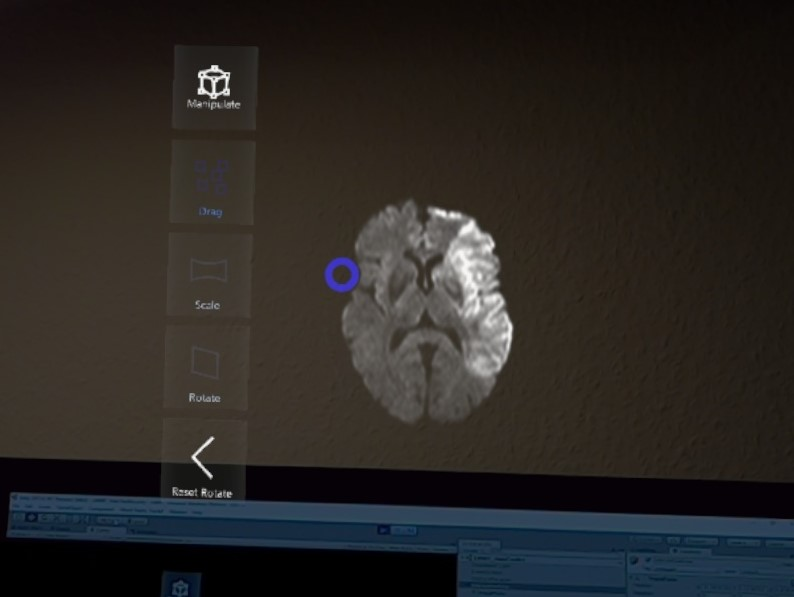
\includegraphics[width=0.5\linewidth]{images/hololens_prototyp.jpg}
	\caption{Aufnahme aus der \textit{HoloLens} von der \textit{HoloLens}-Demo, die Interaktionen ausschließlich über \textit{HoloLens}-Gesten realisiert.}
	\label{img:prototyp}
	\source{Eigene Darstellung}
\end{figure}
\FloatBarrier

\subsection{Positionierung im Raum}
\label{anchor}

Im Kapitel \ref{konzept} wurde bereits erwähnt, dass die dauerhafte Positionierung im Raum, wie sie \textbf{U17} fordert, auf unterschiedliche Weise implementiert werden kann. 
Die \textit{HoloLens} bietet diese Funktionalität in Form von Spatial oder World Anchors. Das Gerät besitzt einen internen Speicher für Anker, die von einer Anwendung angelegt werden, den sogenannten Anchor Store. Durch interne Prozesse bestimmt die \textit{HoloLens} in welchem Raum sie sich gerade befindet. Wird ein World Anchor in diesem Raum abgelegt, wird dessen Standort im Anchor Store gespeichert und behält somit immer seine Position im Raum, auch wenn der Nutzer sich bewegt und über mehrere Sitzungen hinweg. Nachdem ein World Anchor beim Start der Anwendung geladen wird, kann er an ein Objekt, wie ein 3D-Modell anhängt werden, sodass das Objekt an der Position des Ankers dargestellt wird. 

Ohne die Verwendung eines World Anchors wird die 3D-Szene und alle Objekte darin an der \textit{HoloLens} ausgerichtet, die den Nullpunkt der Szene darstellt. Durch die unterschiedliche Ausrichtung kommt es bei der Positionierung der Darstellung in der AR-Anwendung zu Komplikationen, sobald zwischen 2D- und 3D-Szene gewechselt wird. 

Der Anchor Store ist allerdings nur auf der \textit{HoloLens} verfügbar. Wie bereits erläutert wurde, wird die Anwendung im Rahmen dieser Arbeit aber nur auf der \textit{HoloLens} abgespielt, aber nicht für sie bereitgestellt. Dementsprechend ist ein Zugriff auf den Anchor Store nicht möglich. Dasselbe gilt für eine Verwendung der Anwendung in einem VR-System.

Als Alternative dazu können die Daten mit Hilfe eines Markers in den Raum projiziert werden, wie es im Kapitel \ref{grundlagen} beschreiben wurde. \textit{Unity} bietet hierfür das \textit{Vuforia}-Plugin, welches genau das umsetzt. Hierzu können Marker definiert werden, die das Programm erkennt und die diesen zugeordneten GameObjects anzeigt. 
\textit{Vuforia} ist für AR-Anwendungen gedacht und funktioniert durch eine Kamera, die den Marker erkennt. Deshalb kann die Funktion von einer \textit{Vive} nicht genutzt werden, von einer \textit{Vive Pro} jedoch schon, da diese über einen Mixed Reality Modus verfügt. Auch \textit{HoloLens}-Anwendungen können \textit{Vuforia} nutzen. 
Im zeitlichen Rahmen der Arbeit konnte dieses Funktionalität allerdings nicht mehr umgesetzt werden.

\section{Implementierung der Nutzereingabe}

\subsection{Verwendung der \textit{Leap Motion}}

Damit die \textit{Leap Motion} Kamera in einer Anwendung verwendet werden kann, muss das von \cite{orion} zur Verfügung gestellte SDK \textit{Orion} eingebunden werden. Das \textit{Core SDK} ist dabei zur Erkennung und Verwendung des Gerätes notwendig, während ein erweiterndes Paket Funktionen und Beispiele bietet, wie verschiedene Bedienelemente in eine Anwendung integriert werden können, die auf die Controller, also die Hände des Nutzers reagieren.
Meistens funktioniert dies indem einzelne Skripte, die das gewünschte Verhalten implementieren, als Components an GameObjects angehangen werden. Die Skripte lösen dann bestimmte Events oder Methoden aus, die mit den Funktionalitäten der Anwendung verknüpft werden. 

\subsection{Kombination von \textit{Leap Motion} mit \textit{Vive}/\textit{HoloLens}}
\label{kombination}

Sowohl \textit{Vive} als auch \textit{HoloLens} sollen in Verbindung mit der \textit{Leap Motion} funktionieren. Dazu muss zum Einen die \textit{Leap Motion} Kamera in beide Systeme integriert werden und zum Anderen die Funktionalität in die jeweiligen \textit{Unity} Szenen eingebaut werden. 

Das Einbinden der \textit{Leap Motion} in eine VR Anwendung, sowie die Kombination mit dem \textit{Vive} Headset sind unproblematisch. Das \textit{Orion} SDK der \textit{Leap Motion} unterstützt den Einsatz in VR-Szenen. Sofern \textit{SteamVR} installiert und eine VR-Brille angeschlossen ist, ist kein größerer Aufwand nötig, um die Hände des Nutzers in VR anzuzeigen. 
Die Integration in das VR-System ist vergleichbar einfach. Die \textit{Leap Motion} Kamera wird vorne auf dem HMD über der eingebauten Kamera befestigt und ihre Kabel zusammen mit den anderen der Brille über den Kopf des Nutzers geführt. 

Dagegen bringt die Verbindung von \textit{Leap Motion} und \textit{HoloLens} einige Herausforderungen mit sich. Zunächst ist in einer \textit{HoloLens}-Szene nur eine Kamera, die des HMDs, vorgesehen. Das Vorhandensein einer zweiten Kamera, wie die der \textit{Leap Motion} würde beim Erstellungsprozess zu Fehlern führen, sodass das Bereitstellen des Programmes für die \textit{HoloLens} nicht möglich ist.
Die \textit{Leap Motion} wird über ihr Kabel mit Strom versorgt. Sie kann also im Gegensatz zu der \textit{HoloLens} nicht kabellos funktionieren. 
Über das Kabel werden außerdem die von der \textit{Leap Motion} Kamera erfassten Daten weitergeleitet, die dann verarbeitet werden. Die dafür notwendige Software ist nicht für die \textit{HoloLens} verfügbar und es ist fragwürdig, ob sie die dafür notwendige Rechenleistung besitzt. 

Aus diesen Gründen muss die \textit{Leap Motion} während des Betriebs per Kabel mit einem Rechner verbunden sein. Um das Gerät trotzdem in Verbindung mit der \textit{HoloLens} nutzen zu können, müssen entweder die Sensordaten der \textit{Leap Motion} an die Anwendung in der \textit{HoloLens} übertragen werden oder die gesamte Anwendung läuft auf dem Rechner und wird zur Wiedergabe an die \textit{HoloLens} übermittelt. Beides geschieht über Wlan.

Die Übertragung der Sensordaten ist dabei um einiges aufwändiger und erfordert die Integration weiterer Tools. Es existieren einige Lösungsansätze für dieses Problem, beispielsweise von \cite{hololensGithub}. Auf Grund des beschränkten Zeitraums dieser Arbeit wurde dieser Ansatz allerdings nicht implementiert.
Stattdessen wird die Anwendung lediglich auf der \textit{HoloLens} wiedergegeben. Dazu wird die \textit{Hololens}-App \textit{Holographic Remoting Player} von \cite{remoteApp} genutzt. Die Anwendung wird dabei direkt aus dem \textit{Unity}-Editor übertragen.
Die Wiedergabequalität der Anwendung ist dabei abhängig von der Stabilität der Wlan-Verbindung.

Auch das Anbringen der \textit{Leap Motion} an das HMD ist bei der \textit{HoloLens} umständlicher als bei der \textit{Vive}. 
Da die \textit{Vive} einen undurchsichtigen Bildschirm besitzt, kann die \textit{Leap Motion} Kamera einfach vorne auf der Brille befestigt werden. Die Form des Gerätes bietet dazu ausreichend Fläche.
Bei der \textit{HoloLens} sollte der Bildschirm, durch den der Nutzer sieht nicht verdeckt werden. Eine Installation im oberen Teil der Frontseite ist ebenfalls nicht umsetzbar, da dieser von den \textit{HoloLens}-Kameras eingenommen wird, die die Umgebung und Nutzergesten verfolgen.
Somit ist die einzige sinnvolle Möglichkeit, die \textit{Leap Motion} auf der \textit{HoloLens} zu platzieren. Hierbei muss sie außerdem nach vorne geneigt werden, um die Hände des Nutzers in der Anwendung möglichst genau an den realen Händen auszurichten. 

% Ergebnisse


%\chapter{Ergebnisse}
\section{Ergebnisse}
\label{ergebnisse}

Die VR-Anwendung ist als ausführbare Datei im Ergänzungsmaterial zu finden. Da die \textit{HoloLens}-Anwendung, wie in Kapitel \ref{konzept} erläutert, nicht für diese bereitgestellt werden konnte, existiert hierfür keine ausführbare Datei. Allerdings wurde in der ReadMe.txt Datei des Projektes, welches sich ebenfalls im Ergänzungsmaterial befindet beschrieben, wie die Anwendung auf der \textit{HoloLens} abgespielt werden kann. 
Weiterhin ist dort ein Video enthalten, das die Funktionen und Bedienung der Anwendung zeigt.
Die Interaktionslemente wurden wie in Kapitel \ref{konzept} beschrieben implementiert. Neben ihrer Beschreibung sind dort auch Abbildungen der Benutzerelemente zu finden. 


\subsection{3D-Darstellung}

In Abschnitt \ref{3dImplementierung} wurde erläutert, wie die 3D-Darstellung mit Hilfe von Volume Raycasting erzeugt wurde. 
Dazu wurde der Alphawert einer Transfertextur genutzt, um das Rauschen in der Umgebung des Gehirns zu entfernen und die Gehirnform eindeutiger herauszustellen. Dies führt allerdings auch zu Artefakten, dem sogenannten Holzmaserungseffekt. Da allerdings die Darstellung der inneren Strukturen des Gehirns im Vordergrund steht, wurde sich für eine Darstellung entschieden, die durch Reduzierung der Umgebung den Fokus auf das Gehirn erlaubt. 
Im Abbildung \ref{img:resultsDWI} sind die beiden Datensätze mit und ohne die Verwendung einer Transferfunktion abgebildet. Durch Manipulation der Intensität kann bestimmt werden, in welcher Opazität das Gewebe gerendert werden soll, was vor allem das äußere Gewebe beeinflusst. Die Intensität der Renderings in der Abbildung ist in allen Fällen gleich.
Es ist anzumerken, dass die Qualität der Daten sich unweigerlich auf die Qualität des Renderings auswirkt. Die vorgegebenen Datensätze des Gehirns weisen ein hohes Maß an Bildrauschen auf. Außerdem wurden die Schichten offenbar in Abständen solcher Größe gescannt, dass die Interpolation zwischen den Schichten Aktefakte ausweist. Auch dies in in Abbildung \ref{img:resultsDWI} zu sehen.

\begin{figure}[!htb]
	\centering
	\includegraphics[width=0.9\linewidth]{images/dwi_results.png}
	\caption{Rendering der zur Verfügung gestellten Datensätze durch den in mARt verwendeten Shader mit gleicher Intensität. a) Datensatz 1 ohne Transferfunktion b) Datensatz 1 mit Transferfunktion c) Datensatz 2 ohne Transferfunktion d) Datensatz 2 mit Transferfunktion}
	\label{img:resultsDWI}
	\source{Eigene Darstellung}
\end{figure}
\FloatBarrier
  
Aus diesem Grund wurden testweise auch andere Daten mit dem selben Shader gerendert. Das Ergebnis ist dabei von besserer Qualität als mit den Gehirndaten. Die Verwendung der Transferfunktion ist nicht notwendig, um die Darstellung deutlicher zu machen. In Abbildung \ref{img:resultsVisMale} ist der Datensatz eines Kopfes mit und ohne Transferfunktion dargestellt.
  
\begin{figure}[!htb]
	\centering
	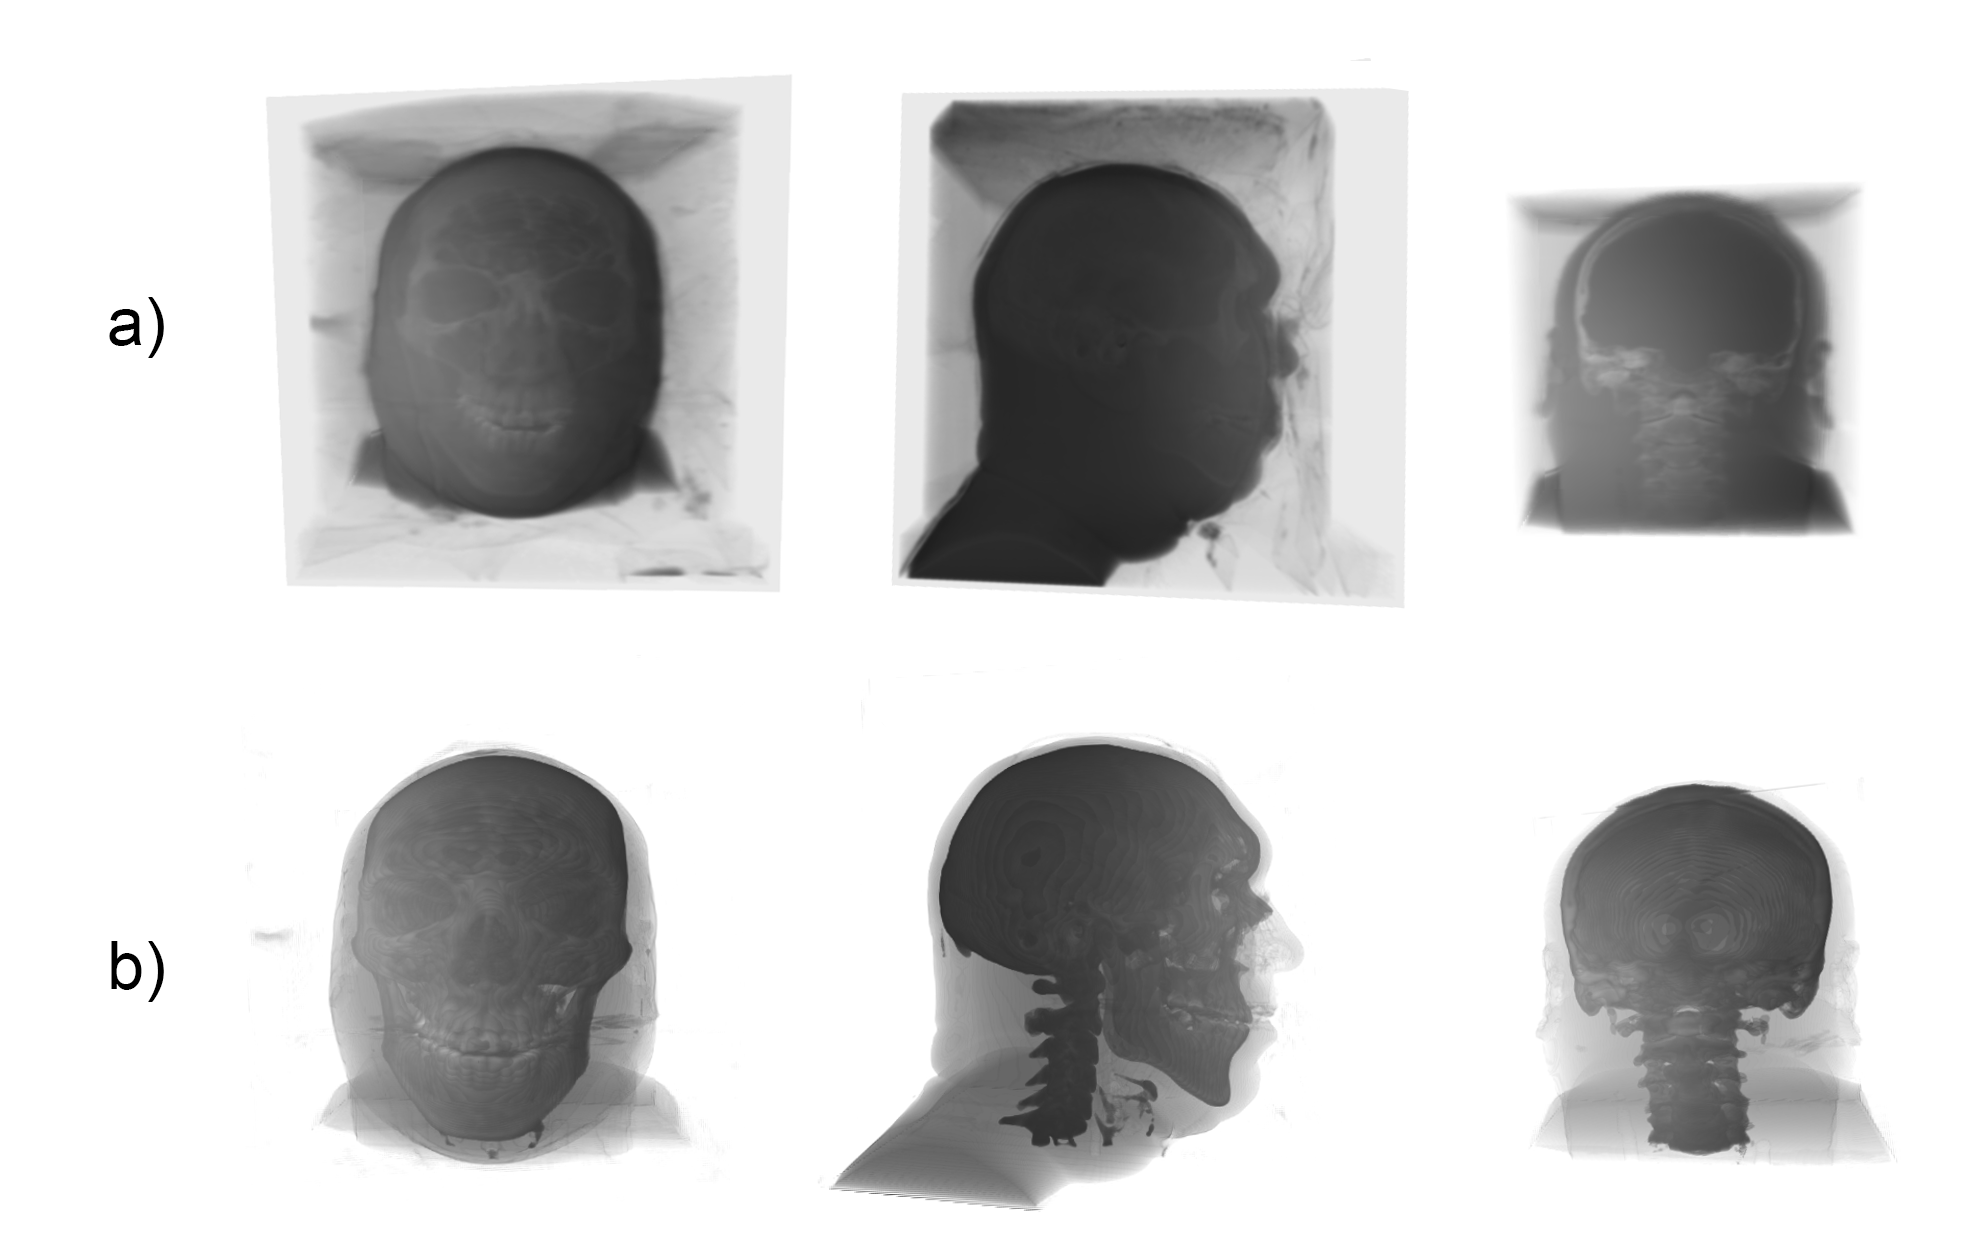
\includegraphics[width=0.9\linewidth]{images/visMale_result.png}
	\caption{Rendering eines alternativen Datensatzes durch den in mARt verwendeten Shader mit gleicher Intensität. a) Rendering ohne Transferfunktion b) Rendering mit Transferfunktion}
	\label{img:resultsVisMale}
	\source{Eigene Darstellung}
\end{figure}
\FloatBarrier

Der gekennzeichnete Bereich, der verdeutlicht welche Teile des Gehirns von dem Schlaganfall betroffen wurden, ist durch die semitransparente Darstellung von allen Seiten gut zu erkennen. 
Durch die Multiplikation der Masken- und Isowerte ist die Struktur des Gehirns weiterhin erkennbar. In Abbildung \ref{img:resultMask} sind Renderings des Gehirns und des Bereichs dargestellt.

\begin{figure}[!htb]
	\centering
	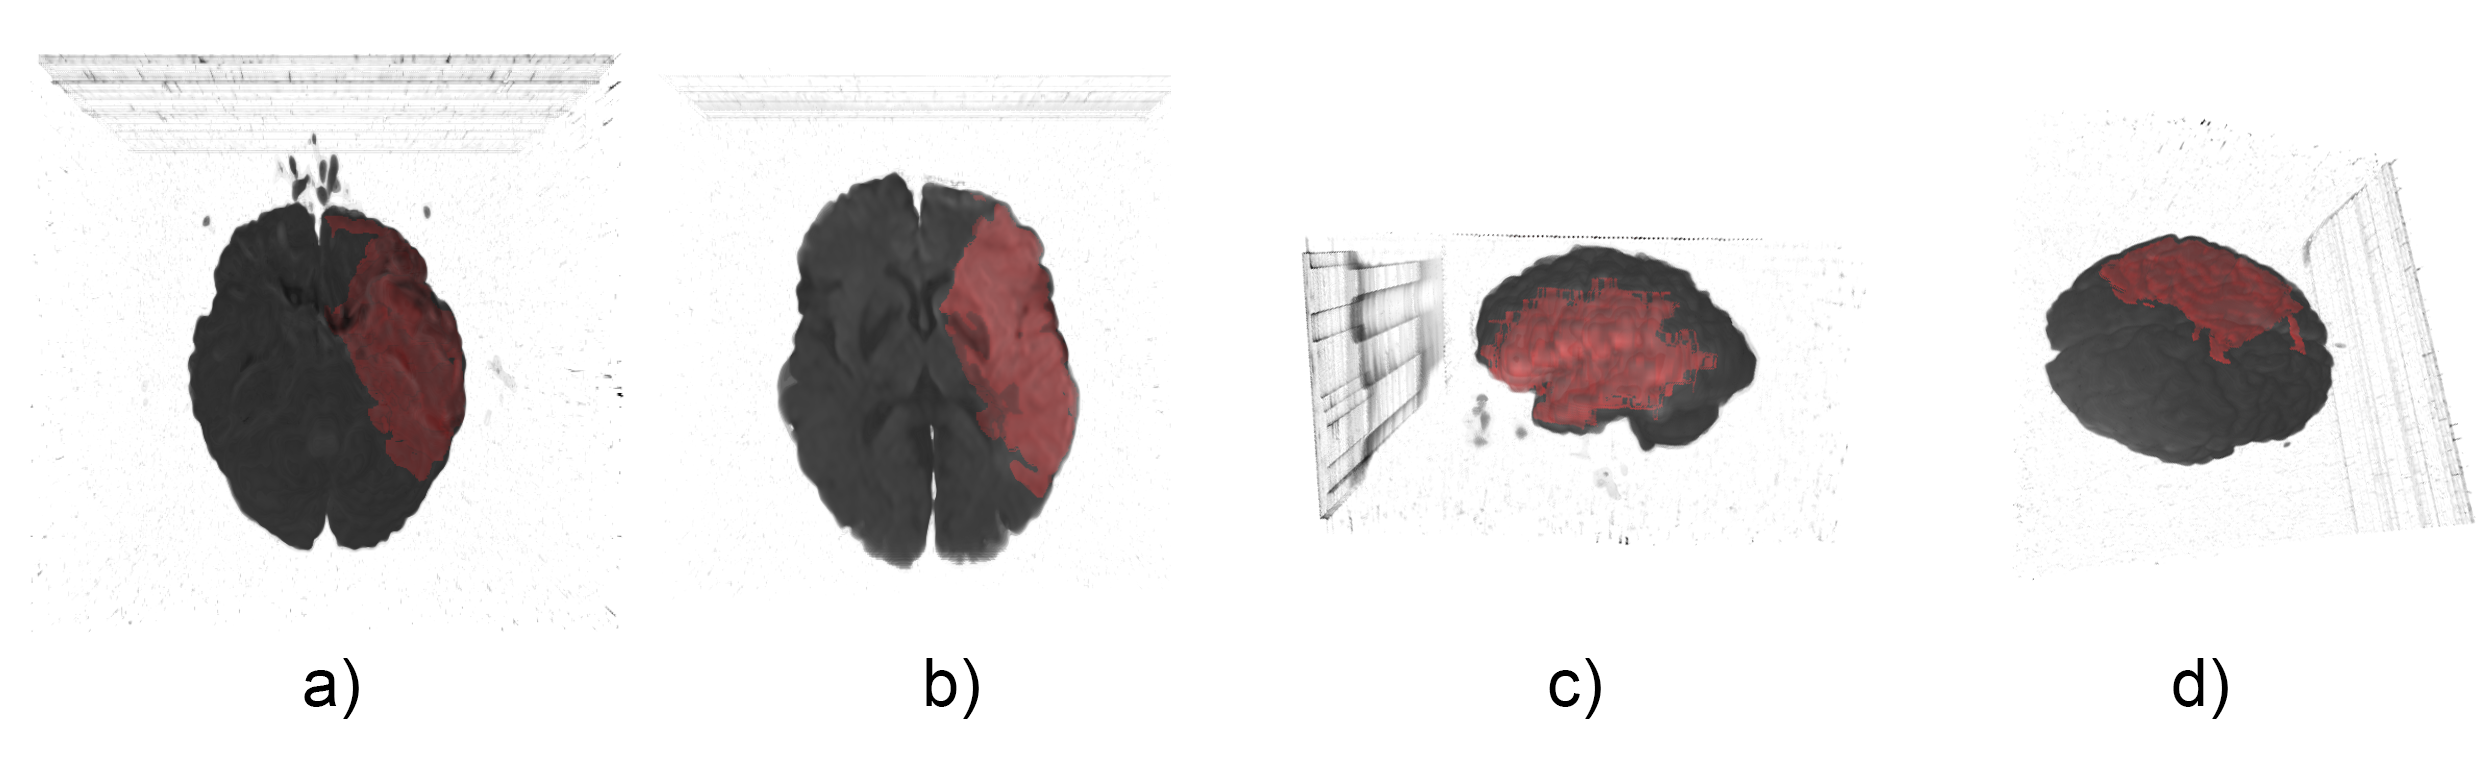
\includegraphics[width=0.99\linewidth]{images/mask_results.png}
	\caption{Rendering des ersten Datensatzes und der Maske, die den betroffenen Bereich hervorhebt, aus verschiedenen Ansichten.}
	\label{img:resultMask}
	\source{Eigene Darstellung}
\end{figure}
\FloatBarrier
  
\subsection{AR Anwendung}
Durch die semi-transparente Darstellung in AR sind die eher dunklen MRT-Daten teilweise schlecht zu erkennen. Dies betrifft vor allem die 3D-Darstellung. Um das Rendering erkennen zu können müssen die Farbwerte durch die Gammakorrektur erhellt werden. In Abbildungen \ref{img:ARLicht} und \ref{img:ARLicht3D} dargestellt, wie die Daten mit dem Standardhelligkeitswert und mit einem erhöhten Wert aussehen.

\begin{figure}[!htb]
	\centering
	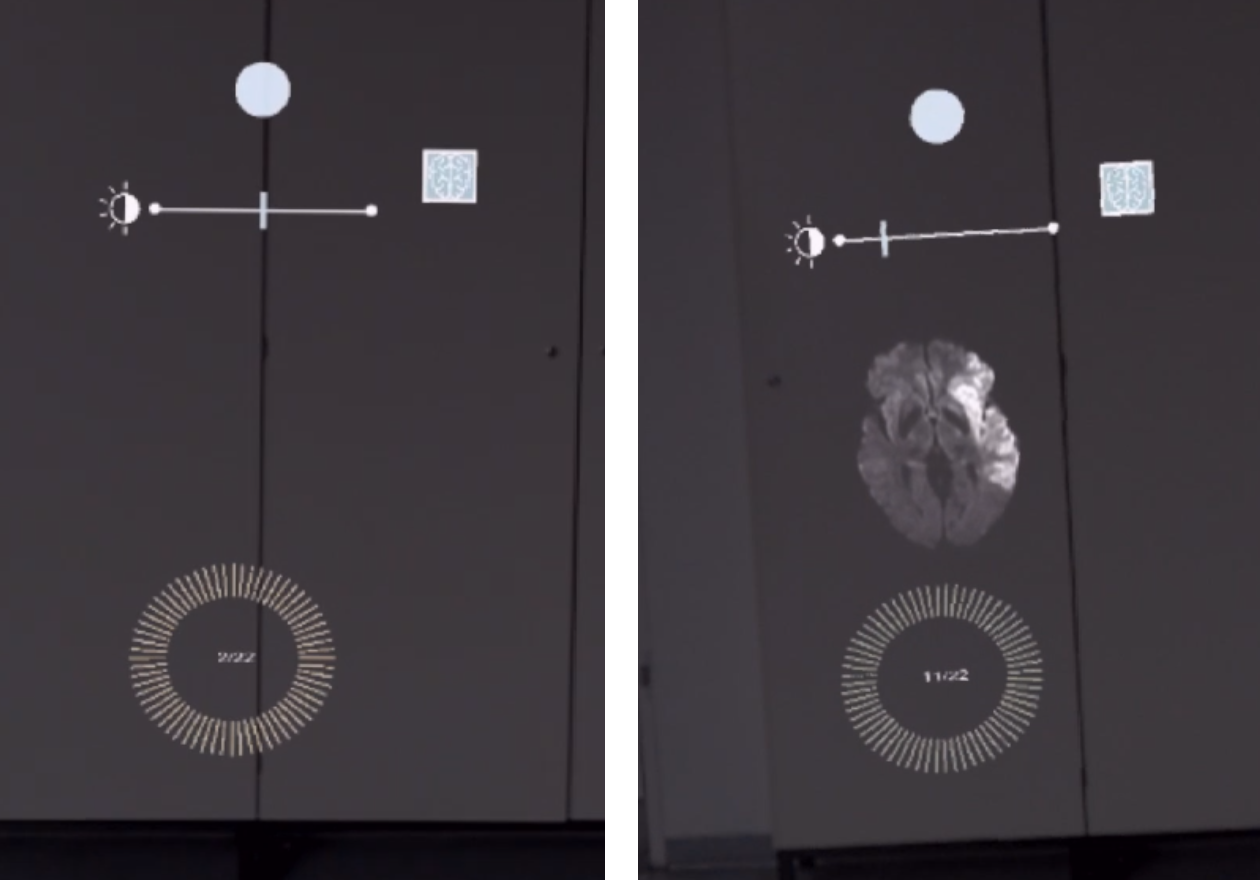
\includegraphics[width=0.7\linewidth]{images/mARt_AR_brightness.png}
	\caption{Zwei Aufnahmen aus der \textit{HoloLens}, während der 2D-Scene von mARt mit unverändertem (links) und erhöhtem (rechts) Gammakorrekturwert. Um die Darstellung erkennen zu können muss der Wert erhöht werden.}
	\label{img:ARLicht}
	\source{Eigene Darstellung}
\end{figure}
\FloatBarrier

\begin{figure}[!htb]
	\centering
	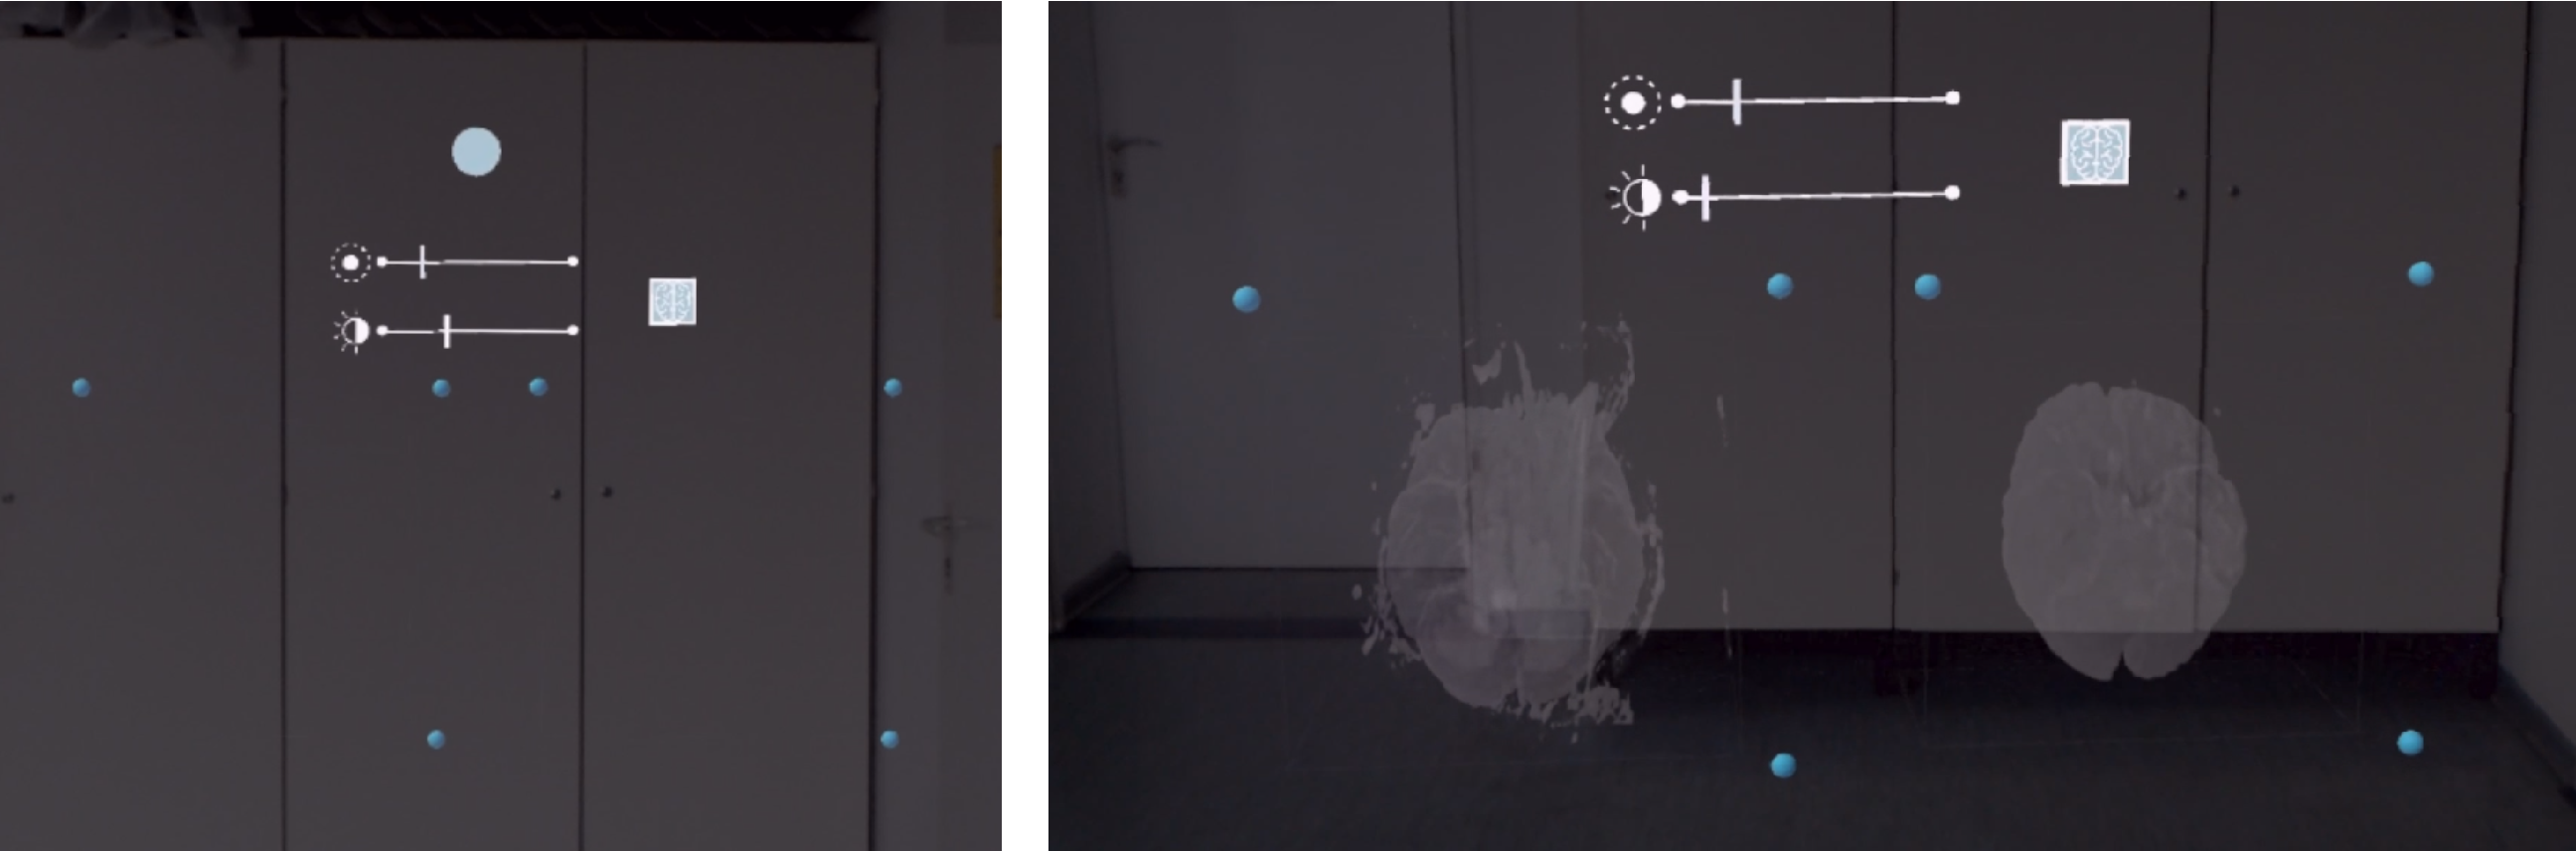
\includegraphics[width=0.9\linewidth]{images/mARt_AR_brightness_3D.png}
	\caption{Zwei Aufnahmen aus der \textit{HoloLens}, während der 3D-Scene von mARt mit unverändertem (links) und erhöhtem (rechts) Gammakorrekturwert. Um die Darstellung erkennen zu können muss der Wert erhöht werden.}
	\label{img:ARLicht3D}
	\source{Eigene Darstellung}
\end{figure}
\FloatBarrier

Ein weiterer Punkt, der die Verwendung der Anwendung auf der \textit{HoloLens} erschwert, ist das eingeschränkte Sichtfeld des Gerätes. Dieses Problem wurde bereit in Kapitel \ref{grundlagen} beschrieben. 
Die Begrenzung der Darstellung führt dazu, dass die MRT-Daten aus der Sicht des Nutzers meist abgeschnitten sind. Um die Daten gleichzeitig mit den Interaktionselementen sehen zu können, muss der Nutzer einen Abstand von ca. 1,5m zur Darstellung haben. Dies macht es ihm allerdings unmöglich mit dieser zu interagieren. Um die Darstellung manipulieren zu können, muss er also zwischen MRT-Bildern und Bedienelementen hin- und herblicken. In Abbildung \ref{img:ARCutoff} ist das abgeschnittene Sichtfeld der \textit{HoloLens} dargestellt. Dabei werden die virtuellen Hände des Nutzer nicht angezeigt, wenn er diese nicht direkt ansieht, auch wenn die Leap Motion diese vielleicht noch erfasst. 
Die Darstellung der Hände selbst nimmt bereits einen großen Teil des Sichtfeldes der \textit{HoloLens} ein, da sie sich nah am HMD befinden. 
Eine Bedienung der Anwendung auf der \textit{HoloLens} ist aus diesen Gründen sehr schwer. 

\begin{figure}[!htb]
	\centering
	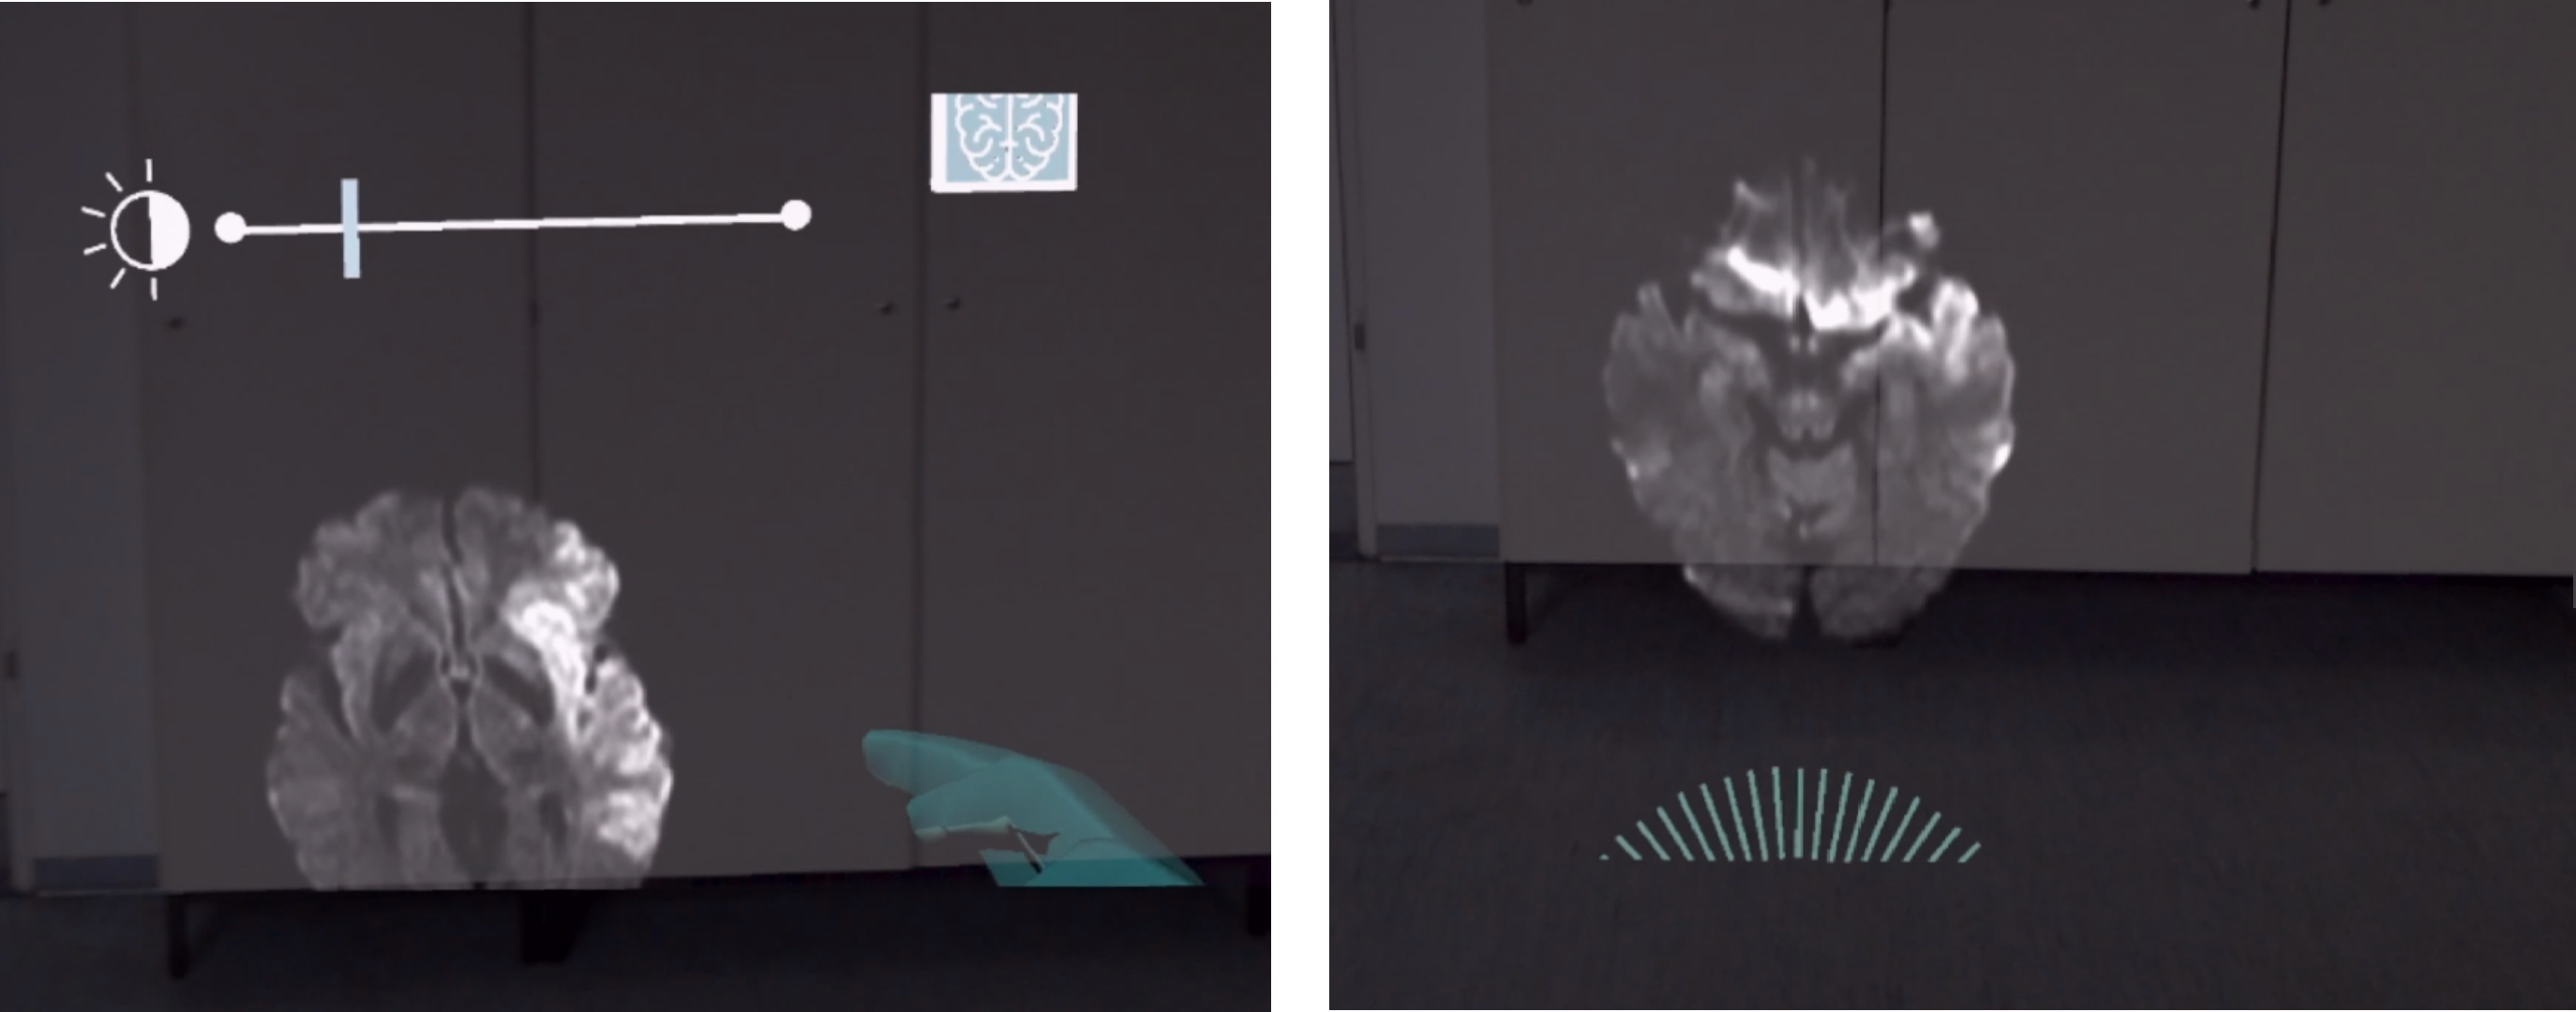
\includegraphics[width=0.9\linewidth]{images/mARt_Cutoff.png}
	\caption{Zwei Aufnahmen aus der \textit{HoloLens}, während der 2D-Scene von mARt aus bedienbarer Entfernung. Durch das begrenzte Sichtfeld der \textit{HoloLens} wir nur ein Ausschnitt der Anwendung dargestellt.}
	\label{img:ARCutoff}
	\source{Eigene Darstellung}
\end{figure}
\FloatBarrier


% Evaluation


\chapter{Evaluation}
\label{evaluation}

\section{Vergleich mit Anforderungen}

Zunächst werden in der folgenden Tabelle \ref{tab:evaluation} die implementierten Funktionen von mARt mit den in Kapitel \ref{anforderung} aufgestellten Anforderungen abgeglichen. Die Anforderung ist dabei über die entsprechende User Story referenziert. Dazu ist angegeben, inwiefern die Anforderung erfüllt wurde, so wie eventuelle Anmerkungen. 

\begin{longtable} {p{.125\textwidth}p{.225\textwidth}p{.60\textwidth}}
\toprule
User Story & Erfüllung & Anmerkungen \\
\toprule
U01 & Erfüllt & Die Darstellung der Daten ist zu großen Teilen abhängig von diesen selbst. Die Darstellung in AR ist abhängig von den Lichtverhältnissen.\\
\midrule 
U02 & Erfüllt & Die Betrachtung aus einem Winkel ist möglich.\\
\midrule 
U03 & Erfüllt & \\
\midrule 
U04 & Erfüllt & Die Anzahl der angezeigten Datensätze ist auf zwei beschränkt.\\
\midrule 
U05 & Erfüllt & Die Daten, aus denen der Nutzer wählen kann sind fest in das Programm integriert und es kann nur aus zwei Datensätzen gewählt werden.\\
\midrule
U06 & Erfüllt erfüllt & Maximal zwei Darstellungen können gleichzeitig manipuliert werden. \\
\midrule 
U07 & Erfüllt & Die zweidimensionale Darstellung kann auf einer Achse verändert werden. Die dreidimensionale auf drei.\\
\midrule 
U08 & Offen & \\
\midrule 
U09 & Erfüllt & \\
\midrule 
U10 & Teilweise erfüllt & Manipulationen außer Skalierung und Rotation werden übernommen, sofern der Wert in beiden Szenarien existiert.\\
\midrule 
U11  & Erfüllt & \\
\midrule
U12 & Erfüllt & Eine Manipulation der Maske würde dem Nutzer eine Anpassung erlauben, wurde jedoch nicht umgesetzt.\\
\midrule 
U13 & Erfüllt & \\
\midrule 
U14 & Erfüllt & \\
\midrule 
U15 & Erfüllt & Nur bei Anzeige eines Datensatzes möglich. Temporäte Manipulation.\\
\midrule 
U16 & Erfüllt & Die position wird nicht über mehrere Sitzungen hinweg gespeichert.\\
\midrule 
U17 & Offen & Nicht umsetzbar durch Abhängigkeit von einem PC.\\
\midrule 
U18 & Offen & Keine unterschiedlichen Sequenzen standen zur Verfügung.\\
\midrule 
U19 & Offen & Datensätze sind in Anwendung integriert.\\
\midrule 
U20 & Offen & Datensätze sind in Anwendung integriert.\\

\bottomrule
\caption{\label{tab:evaluation}Erfüllung der Anforderungen.}
\end{longtable}

\section{Nutzertest}

Um die Verwendung von mARt im Bereich der Schlaganfallbehandlung zu evaluieren wurde ein Nutzertest abgehalten. 
Dabei wurden sowohl die AR- als auch die VR-Anwendung von einem Neurologen getestet. 

Ergebnisse

\section{Auswertung}
% Was ist besser als vorher? Warum?
% Fazit

\chapter{Zusammenfassung und Fazit}
\label{fazit}

\section{Zusammenfassung}

Im Rahmen dieser Arbeit wurde untersucht, inwiefern eine interaktive dreidimensionale Darstellung von MRT-Daten in einer AR-Anwendung einen Mehrwert für Neurologen im Bereich der Behandlung von Schlaganfällen bietet. 
Hierzu wurden zunächst technische Hintergründe zu MRT-Daten, den Möglichkeiten der 3D-Darstellung von diesen sowie AR- und VR-Technologien erläutert. Weiterhin wurden damit in Zusammenhang stehende Arbeiten genannt. Einer der Schwerpunkte dieses Abschnitts war die Vorstellung verschiedener Volume Rendering Techniken.

Als Grundlage zur Konzeption der AR-Anwendung wurden dann Anforderungen aufgestellt, die durch Interviews mit einem Neurologen der Charité Berlin erarbeitet wurden. Diese wurden als User Stories formuliert.

Anschließend wurde diskutiert, wie die einzelnen Funktionalitäten von mARt umgesetzt werden können. Hierbei wurden sowohl Aspekte der Implementierung als auch der Gestaltung von Bedienelementen und Aussehen der Anwendung berücksichtigt. Unter anderem wurden aus den zuvor beschriebenen Techniken die geeignetsten ausgewählt. 

Das beschriebene Konzept wurde implementiert und einzelne relevante Punkte der Umsetzung wurden erläutert. Die Ergebnisse der Implementierung wurden präsentiert.

Schließlich wurde die Anwendung mit den zuvor aufgestellten Anforderungen abgeglichen und von einem Neurologen getestet. 
Es konnte gezeigt werden, dass die Darstellung der dreidimensionalen Daten im Raum zu einem besseren Verständnis der Situation führt. Die direkte Interaktion mit der Darstellung trägt dazu bei. 

\section{Ausblick}

Wie mehrfach beschrieben wurde, handelt es sich bei mARt primär um einen Prototyp, der die Vorteile des Einsatzes einer AR-Anwendung zur Darstellung von MRT-Daten untersucht. Dementsprechend existieren viele Möglichkeiten das Programm in verschieden Richtungen zu erweitern.
Im Folgenden werden einige mögliche weiterführerende Entwicklungen von mARt erläutert.

\subsection{Implementierung offener  Anforderungen}

Wie im Kapitel \ref{evaluation} dargelegt wurde, konnte nicht alle anfangs gestellten Anforderungen im Rahmen dieser Arbeit umgesetzt werden. Um mARt für den Einsatz im Arbeitsumfeld nutzbar zu machen sollten diese erfüllt sein.

%U08
In User Story \textbf{U08} wird ein Scrollrad für den Wechsel zwischen den Schichten gefordert. Da die Steuerung von mARt im Rahmen dieser Arbeit allerdings durch Gesten erfolgt, wurde sie nicht erfüllt. In zukünftigen Konzepten lässt sich die Gestensteuerung allerdings möglicherweise mit anderen Bedienelementen kombinieren, beispielsweise einem Scrollrad, das multifunktional verwendet wird. Dies ist allerdings abhängig von dem angestrebten Anwendungsfall.

%U10 (teilweise)
Weiterhin wurde durch Story \textbf{U10} ein Wechsel zwischen 2D- und 3D-Darstellung beschrieben, bei dem die vom Nutzer getätigten Manipulationen in das jeweils andere Szenario übertragen werden. Diese Anforderung wurde nur teilweise erfüllt. Wie in Kapitel \ref{konzept} erläutert wurde, sind manche Manipulationen, wie die Skalierung nur temporär. In einem veränderten Konzept einer AR-Anwendung wie mARt, können sich Möglichkeiten ergeben alle Manipulationen zu übertragen oder sogar die Darstellungen synchron anzuzeigen.

%U17
Die in Story \textbf{U17} geforderte dauerhafte Positionierung im Raum wurde ebenfalls nur teilweise umgesetzt. Die Darstellung kann im Raum platziert werden. Allerdings behält sie diese Position nicht über mehrere Sitzungen hinweg. 
Weiterhin ist ihre Position relativ zur Position des Nutzers. Für den Prototyp ist dies ausreichend. Die User Story hat ihren Ursprung allerdings in der Idee einer Multiuser-Anwendung. Dabei können mehrere Nutzer die selbe Darstellung betrachten, die sich für alle an der selben Position im Raum befindet. Dieses Konzept wurde in Kapitel \ref{konzept} erläutert. Vor allem für Einsätze demonstrativer Art, wie Lernzwecke oder die Kommunikation mit Patienten wäre diese Funktion von Nutzen.

%U18
Eine weitere unerfüllte User Story ist \textit{U18}, die beschreibt, dass möglichst alle Sequenzen eines Scans eines Patienten wählbar sein sollen. Für diese Arbeit wurden nur eine begrenzte Anzahl an Datensätzen zur Verfügung gestellt. Bei der Untersuchung eines möglichen Schlaganfalls, kommen allerdings oft verschiedene Scans und Gewichtungen zum Einsatz, wie in Abschnitt \ref{mrt} beschrieben wurde. Sollten mehrere Datensätze zu einem Patienten vorliegen, ist es sinnvoll aus diesen wählen zu können. Dies steht allerdings in Zusammenhang mit der Implementierung einer generellen Auswahl von Daten, aus denen der Nutzer wählen kann, wie sie bereits dargelegt wurde.

%U19-20
Wie ebenfalls in Kapitel \ref{konzept} erläutert wurde, unterstützt der Prototyp nicht die Darstellung von vom Nutzer gewählten Dateien. Dementsprechend werden auch keine Dateien im DICOM- oder NIfTI-Format unterstützt. Für die Nutzung von Neurologen oder auch erweiterte Tests ist diese Funktion allerdings notwendig. Dazu müsste im Konzept der Anwendung eine Möglichkeit gefunden werden dem Nutzer die Auswahl von Daten zu erlauben und diese in das Programm zu übertragen. Dies setzt unter anderem voraus, dass ein Parser integriert wird, der die Daten aus besagten Formaten in einen für \textit{Unity} lesbaren Typ umwandelt. 

Hinzu kommen die Erweiterungen, die in Abschnitt \ref{nutzertest} beschrieben wurden. 
Abhängig von den konkreten Nutzungsszenarien werden sich außerdem weitere Anforderungen ergeben, um die mARt erweitert bzw. an die es angepasst werden muss. 
Es wäre wünschenswert, dass diese sowie zukünftige ähnliche Arbeiten einem Test mit einer größeren Anzahl an Testern unterzogen wird, da dies noch mehr Aufschluss über die Bedürfnisse verschiedener Nutzer und die Möglichkeiten einer AR-Anwendung liefert.

\subsection{Verbesserte 3D Visualisierung}

Die Ergebnisse des Volume Rendering der MRT-Daten wurde in Abschnitt \ref{ergebnisse} demonstriert. Der Nutzertest hat gezeigt, dass die Darstellungen von ausreichender Qualität sind, um eine Diagnose durchzuführen und vor allem den Zustand des Gehirns nach einen Schlaganfall zu vermitteln. 
Allerdings stellt das Volume Rendering für sich einen eigenen Forschungsbereich dar, der im Rahmen dieser Arbeit nicht abgedeckt werden konnte. Darin existieren viele Maßnahmen, um die Qualität der Darstellung weiter zu verbessern. Einige davon werden an dieser Stelle genannt. 

Zum einen wurde als Rendering Verfahren das Volume RayCasting gewählt, da es sehr gute Ergebnisse liefert. Je nachdem in welche Richtung sich zukünftige Arbeiten entwickeln, ist es allerdings sinnvoll weitere Verfahren zu testen, die beispielsweise weniger rechenintensiv sind. 
Weiterhin wurde zwar eine Transferfunktion verwendet, um das Rauschen der Bilder zu beschränken. Allerdings ist diese nicht für jeden Datensatz optimal und es wird lediglich ihr Alphawert genutzt. 
Idealerweise sollte dem Nutzer die Möglichkeit gegeben werden die Transferfunktion zu beeinflussen, wie es in Kapitel \ref{konzept} bereits erläutert wurde. Dies würde die Darstellungsqualität erhöhen und dem Nutzer zu einem Rendering nach seinen Ansprüchen verhelfen. 
Um das Rendering plastischer und realer erscheinen zu lassen kann außerdem ein globales Beleuchtungsmodell implementiert werden, wie es in Kapitel \ref{grundlagen} beschrieben ist. 
Da die Qualität des Renderings von den Bilddaten abhängt, können diese schließlich bereinigt bzw. aufgearbeitet werden. Wie in Abschnitt \ref{ergebnisse} dargelegt wurde, besteht in den gegebenen Datensätzen ein hohes Maß an Rauschen. Dieses könnte auf verschiedenen Wegen herausgefiltert werden, bevor die Bilder gerendert werden. Zudem könnte eine zusätzliche Interpolation vorgenommen werden, die die großen Abstände zwischen den einzelnen Schichten besser überbrückt als es bisher der Fall ist. Damit könnten Bildartefakte reduziert werden. 
Für die Verbesserung der MRT-Daten könnte beispielsweise maschinelles Lernen eingesetzt werden.

\subsection{Übertragen der Anwendung auf andere Hardware}
\label{hololens2Fazit}

Im Rahmen dieser Arbeit wurde mARt als AR-Anwendung nur auf der \textit{HoloLens} getestet. 
Die Verwendung der Anwendung zusammen mit anderen AR-Systemen, könnte noch mehr Aufschluss über die Möglichkeiten von AR-Systemen im medizinischen Bereich geben. 
mARt könnte dabei auf vergleichbaren AR-Systemen, wie der \textit{Magic Leap} von \cite{magicLeap} getestet werden.
Da die Entwicklung solcher Systeme momentan weiter fortschreitet, kommen allerdings auch noch nicht erschienene Geräte in Betracht.

Wie im Kapitel \ref{evaluation} beschreiben wurde, ist die Interaktion mit mARt durch das geringe Sichtfeld der \textit{HoloLens} erschwert. Die Inhalte werden abgeschnitten und die virtuellen Hände nehmen viel Platz ein. 
Dieses und andere Probleme, die bei der Verwendung von mARt auf der \textit{HoloLens} festgestellt wurden, könnten eventuell durch die Verwendung auf der \textit{HoloLens 2} behoben werden. 
Das Gerät wurde im Februar 2019 vorgestellt und soll voraussichtlich im April 2019 erscheinen. 
Die neue Version der \textit{HoloLens} besitzt ein mehr als doppelt so großes Sichtfeld, wie ihr Vorgänger (vgl. \cite{hololens2}), was dem eben genannten Problem entgegen wirkt. 
Weiterhin verfügt die \textit{HoloLens 2} über eine eingebaute Hand-Tracking-Funktion (vgl. \cite{hololens2}). Diese könnte an Stelle der \textit{Leap Motion} zum Erfassen der Hände des Nutzers verwendet werden. Dadurch entstehen zwei Vorteile gegenüber der aktuellen Anwendung. Zum Einen ist anzunehmen, dass die virtuellen Hände nicht länger angezeigt werden müssen. Dies vereinfacht die Benutzung und lässt mehr Raum im Sichtfeld für tatsächliche Inhalte. Zum Anderen, könnte die Anwendung für die \textit{HoloLens 2} bereitgestellt und somit kabellos verwendet werden, wodurch die Verzögerung der Übertragung auf das Gerät behoben und das Nutzungserlebnis verbessert würden. 

Weiterhin ist davon auszugehen, dass die \textit{HoloLens 2} über eine höhere Rechenleistung verfügt, als ihr Vorgänger. Dies könnte neben der eben genannten Optimierung des Renderingverfahrens eine flüssige Darstellung der 3D-MRT-Daten ermöglichen.

Eine Übertragung der Anwendung auf die \textit{HoloLens 2} könnte die Benutzbarkeit der Anwendung demnach stark erhöhen.

\subsection{Integration anderer Technologien}

Im vorherigen Abschnitt wurde bereits der Einsatz von maschinellem Lernen zur Verbesserung der Bildqualität angeführt. Diese Technologie könnte weiterhin zur Diagnose von Schlaganfällen oder zur Prognose ihrer Entwicklung verwendet werden. Funktionen dieser Art könnten in Anwendungen wie mARt  integriert werden.
\todo{Paper? P}

\section{Fazit}

Die Motivation hinter dieser Arbeit war es zu untersuchen, inwiefern eine interaktive AR-Anwendung die Untersuchung von volumetrischen MRT-Daten verbessern kann. Obwohl der dafür entworfene Prototyp längst nicht den Umfang eines MRT-Viewers abdeckt, konnten Schlüsse über die Möglichkeiten einer solchen Anwendung gezogen werden.
Der Nutzertest hat gezeigt, dass mARt zu einem besseren Verständnis der Situation führen kann. Dies wird durch die dreidimensionale Darstellung im Raum sowie die direkte Interaktion mit den Daten erreicht.
Eine AR-Anwendung dieser Art besitzt enormes Potenzial Nutzer in verschiedenen Anwendungsfällen zu unterstützen. Dazu gehört die Arbeit von Neurologen aber auch anderen Ärzten, sowie das Studium von Medizinstudenten und die Kommunikation mit Patienten. 

Bis AR-Anwendungen wie mARt Alltagsrealität werden bedarf es allerdings noch weiterer Entwicklungen.
Der derzeitige Stand der AR-Technologie stellt dabei das größte Hindernis dar. Wie in der Arbeit gezeigt werden konnte, ist die Darstellung von Volumendaten ein weitreichend erforschtes Gebiet. Um eine solche Darstellung über ein HMD in einer interaktiven Anwendung zur Verfügung zu stellen, muss dieses drei Voraussetzungen erfüllen:

\begin{itemize}
\item Die Leistung muss ausreichen, um hochwertige Renderings durchzuführen.
\item Es müssen intuitive und bequeme Interaktionsmöglichkeiten verfügbar sein.
\item Der Tragekomfort sollte eine Benutzung über einen längeren Zeitraum ermöglichen.
\end{itemize}

All dies trifft momentan nicht auf AR-HMDs wie die \textit{HoloLens} zu. Es ist wahrscheinlich, dass zukünftige Systeme der ständig voranschreitenden Technologie diese Eigenschaften mitbringen werden. 
Bis dahin gilt es zu untersuchen, was die notwendigen Interaktionen und relevantes Elemente für die jeweiligen Anwendungsfälle sind und wie diese sinnvoll in AR realisiert werden können, damit eine stabile und einsetzbare Anwendung entstehen kann, die das dargelegte Potenzial ausschöpft.
mARt ist somit der erste Schritt einer Entwicklung, um die Arbeit und Zusammenarbeit von Ärzten, Studenten und Patienten zu bereichern.



\pagebreak

\printbibliography

\end{document}
